\chapter{Score-Based Perspective: From EBMs to NCSN}\label{ch:score-based}

% In the previous chapters we traced diffusion models back to their variational roots, showing how they emerge from the framework of VAEs. We now turn to a second, equally fundamental view-point: \emph{Energy-Based Models (EBMs)}. EBMs describe data distributions through unnormalized energy functions, and by examining their gradients we arrive at the notion of a \emph{score function}. This chapter builds the bridge from EBMs to what will later crystallize as \emph{score-based diffusion models}. For readers already versed in EBMs, this section serves as a focused refresher and a stepping stone toward the score-based view.

In the previous chapters we traced diffusion models to their variational roots and showed how they arise within the framework of VAEs. We now turn to a second, equally fundamental viewpoint: \emph{Energy-Based Models} (EBMs)~\citep{ackley1985learning,lecun2006tutorial}. An EBM represents a distribution by an energy landscape that is low on data and high elsewhere. Sampling typically relies on Langevin dynamics, which moves samples toward high density regions by following the gradient of this landscape. This gradient field, known as the \emph{score}, points toward directions of higher probability.

The central observation is that knowing the score is enough for generation: it moves samples toward likely regions without computing the intractable normalization constant. \emph{Score-based} diffusion models build directly on this idea. Instead of focusing only on the clean data distribution, they consider a sequence of Gaussian noise–perturbed distributions whose scores are easier to approximate. Learning these scores yields a family of vector fields that guide noisy samples step by step back to data, turning generation into progressive denoising.


\chapterlearning{
  \item understand the core idea of score-based modeling: what a score function is, and how it can be used with Langevin dynamics for generation;
  \item understand how denoising score matching learns the score at a single noise level through conditioning trick, and how Tweedie's formula connects score prediction to denoising;
  \item understand how Noise Conditional Score Networks (NCSNs) extend denoising score matching to multiple noise levels, why multiple noise levels are useful, and how NCSN score prediction relates to DDPM noise prediction.
}{
Readers already familiar with energy-based models may skim \Cref{sec:ebm} and begin with \Cref{subsec:training-sm}.
}

% \se{fix language, ideally give some intuition for this connection}

\newpage


\section{Energy-Based Models}\label{sec:ebm}

For readers already familiar with EBMs, this section is meant as a concise refresher and a bridge to the score-based view of diffusion.
\subsection{Modeling Probability Distributions Using Energy Functions}

Let $\mathbf{x} \in \mathbb{R}^D$ denote a data point. EBMs define a probability density via an energy function $E_{\bm{\phi}}(\mathbf{x})$, parameterized by ${\bm{\phi}}$, which assigns lower energy to more likely configurations. The resulting distribution is given by
\begin{align*}
    p_{{\bm{\phi}}}(\mathbf{x}) := \frac{\exp(-E_{\bm{\phi}}(\mathbf{x}))}{Z_\bphi}, \quad 
    Z_\bphi := \int_{\mathbb{R}^D} \exp(-E_{\bm{\phi}}(\mathbf{x})) \diff\mathbf{x},
\end{align*}
where $Z_\bphi$ is called the \emph{partition function} ensuring normalization:
\[
\int_{\mathbb{R}^D} p_{{\bm{\phi}}}(\mathbf{x})  \diff\mathbf{x} = 1.
\]
\begin{figure}[th!]
    \centering
    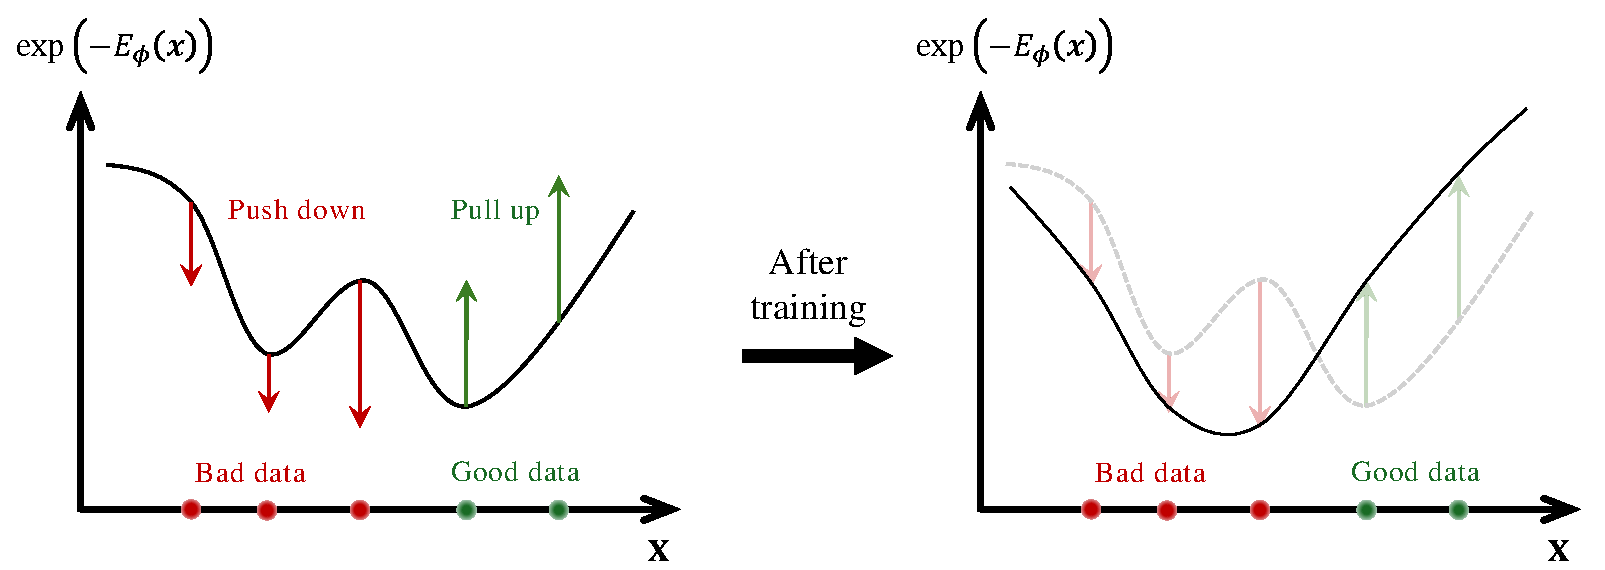
\includegraphics[width=\linewidth]{Images/PartB/ebm-graph.pdf}
    \caption{\textbfs{Illustration of EBM training.} The model lowers density (raises energy) at ``bad'' data points (red arrows), and raises density (lowers energy) at ``good'' data points (green arrows). \figcredit{Created by the authors.}}
    \label{fig:ebm-graph}
\end{figure}



In this view, points with lower energy correspond to higher probability, much like a ball rolling down into a valley. The partition function $Z_{\bphi}$ ensures that all probabilities add up to one, and as a result only the \emph{relative} values of energy matter. For instance, adding a constant to all energies multiplies both numerator and denominator by the same factor, leaving the distribution unchanged. 

Moreover, because the partition function $Z_{\bphi}$ enforces that probabilities sum to one, it follows mathematically that decreasing the energy within a region increases its probability, while the probability of its complement decreases accordingly. Thus, EBMs obey a strict global trade-off: making one valley deeper inevitably makes others shallower, and probability mass is redistributed across the entire space rather than assigned independently to each region.


\paragraph{Challenges of Maximum Likelihood Training in EBMs.}
In principle, EBMs can be trained by maximum likelihood, which naturally balances fitting the data with global regularization (see \Cref{eq:MLE}):
\begin{align}
\label{eq:mle-ebm}
\mathcal{L}_{\text{MLE}}(\bphi) 
&= \mathbb{E}_{p_{\text{data}}(\rvx)}  \left[ \log \frac{\exp(-E_{\bphi}(\rvx))}{Z_\bphi} \right] \\
&= -  \underbrace{\mathbb{E}_{p_{\text{data}}}[E_{\bphi}(\rvx)]}_{\text{lowers energy of data}}
   -  \underbrace{\log \int \exp(-E_{\bphi}(\rvx))\diff\rvx}_{\text{global regularization}}, \nonumber
\end{align}
with $Z_\bphi = \int \exp(-E_\bphi(\rvx))\diff\rvx$. 
The first term lowers the energy of real data, while the second enforces normalization via the partition function.

However, in high dimensions computing $\log Z_{\bphi}$ and its gradient is intractable, as it requires expectations under the model distribution. 
This motivates alternative objectives that either approximate the term, such as contrastive divergence \citep{hinton2002training}, or avoid it altogether through \emph{score matching}. 

In what follows, we first introduce the notion of the score function in \Cref{subsec:motivation-score} and present score matching as a tractable training objective that bypasses the partition function in \Cref{subsec:training-ebm}, and then discuss Langevin dynamics as a practical sampling method with score functions in \Cref{subsec:sampling-ebm}. 

% \paragraph{Preface: Efficient EBM Training via Score Matching.}


% \paragraph{Preface: Sampling via Score Functions.}
% Training alone is not sufficient; EBMs must also generate samples from their learned energy landscape. 
% Since they lack an explicit generator, this is typically achieved with Markov Chain Monte Carlo methods. 
% Among these, \emph{Langevin dynamics} is particularly effective: it updates samples using only the gradient of the energy (the score function), 
% guiding them toward regions of higher probability and enabling efficient sampling without computing the partition function.









% \paragraph{Intuition Behind Energy-Based Models.}
% \jcr{Drawing from the physical analogy of a ball gravitating towards a low-energy valley, Energy-Based Models (EBMs) define a distribution by assigning an \emph{energy} $E_\bphi(\rvx)$ to each point $\rvx$ and converting these values into probabilities $p_\bphi(\rvx) = \tfrac{\exp(-E_\bphi(\rvx))}{Z_\bphi}$. Lower energy means larger $\exp(-E_\bphi(\rvx))$ and thus higher probability mass, so regions where the energy landscape forms deep valleys correspond to more likely and realistic data. The partition function $Z_\bphi$ ensures proper normalization, since $\exp(-E_\bphi(\rvx))$ alone does not integrate to one. Importantly, only relative energies matter: adding a constant $c$ shifts both numerator and denominator by the same factor $e^{-c}$, leaving $p_\bphi$ unchanged.

% This normalization induces a global trade-off across the space. To see this, consider a region $A$, where its probability under $p_\bphi$ is
% \[
% \frac{\int_A \exp(-E_\bphi(\rvx)) \diff\rvx}{\int \exp(-E_\bphi(\rvx)) \diff\rvx} = \frac{\int_A \exp(-E_\bphi(\rvx)) \diff\rvx}{\int \exp(-E_\bphi(\rvx)) \diff\rvx}.
% \]
% If $E_\bphi$ is decreased on $A$, the numerator grows and thus the probability on $A$ increases. Since the denominator grows as well, the relative weight of the complement $A^c$ must shrink so that the total probability remains one. In plain words, making one valley deeper necessarily makes other valleys shallower, because $Z_\bphi$ redistributes probability mass across the entire space. This captures the essence of EBMs: the model does not assign probabilities independently to regions, but balances them through a single global normalization.

% }
% % Drawing from the physical notion that systems gravitate towards lower potential energy (e.g., a ball in a valley), Energy-Based Models define a probability distribution by assigning an \emph{energy} $E_\bphi(\mathbf{x})$ to each data point $\mathbf{x}$. Crucially, lower energy corresponds to higher likelihood and more realistic data, while high energy signals low probability, mirroring how physical systems avoid high-energy configurations. This framework allows EBMs to model intricate, multimodal distributions without explicit latent variables or restrictive parametric assumptions, distinguishing them from approaches like VAEs. 
% % The energy function provides a direct, interpretable measure of data plausibility.
% % \se{won't be clear why without mentioning normalization}

% % \se{need to add citations}



% \paragraph{Challenge of Energy-Based Models.}
% Despite their conceptual appeal, EBMs are challenging to train (and actually also sample) due to the intractability of $Z_\bphi$, which involves integrating over the full input space. Consequently, practical methods rely on approximate or surrogate objectives that bypass direct evaluation of the partition function while still encouraging the model to fit the data distribution.


% \paragraph{Naïve Training of Energy-Based Models.}
% \jc{The fundamental goal when training an EBM is to assign low energy to genuine data points, making them highly probable under our model. In theory, one could drive the energy of training samples arbitrarily low, leading to a degenerate `spiky'' density that places almost all probability on the data and ignores the rest of the space. In practice, however, this collapse is prevented by the smooth and finite capacity parameterization of a neural network $E_\bphi$, which, together with the global normalization constraint, discourages sharply concentrated distributions.
% }
% \se{not sure this overfitting discussion is valuable here}
% This trade-off is naturally captured by the maximum likelihood objective (see \Cref{eq:MLE}), which balances data fitting with global regularization:
% \begin{align}
% \begin{aligned}
%     \label{eq:mle-ebm}
%     \mathcal{L}_{\text{MLE}}({\bm{\phi}}) &= \mathbb{E}_{p_{\text{data}}(\mathbf{x})} \left[ \log \frac{\exp(-E_{\bm{\phi}}(\rvx))}{Z_\bphi} \right] \\
%     &= - \underbrace{\mathbb{E}_{p_{\text{data}}(\mathbf{x})} [E_{\bm{\phi}}(\rvx)]}_{\text{pulls down energy of data}} - \underbrace{\log \int_{\mathbb{R}^D} \exp(-E_{\bm{\phi}}(\mathbf{x})) \diff\mathbf{x}}_{\text{global regularization}},
% \end{aligned}
% \end{align}
% where we use the definition of $Z_\bphi=\int \exp(-E_\bphi(\rvx))\diff\rvx$.
% % \se{probably better to spell out the def of the partition function here (integral) so the tradeoff is clear}
% The first term encourages low energy for real samples, while the second term, via the partition function $Z_\bphi$, penalizes spreading low energy too broadly; thus promoting a well-distributed model.

% % However, computing $Z_\bphi$ is generally intractable, as it involves integrating over the entire data space. Consequently, exact maximum likelihood training is rarely feasible in practice. This motivates the use of approximation methods such as \emph{Contrastive Divergence} or alternative objectives like \emph{Score Matching}, which offer tractable estimates of the gradient. \se{add citations. tie to the divergence discussion in early chapters?}


% \jcr{
% While conceptually simple, evaluating the partition function $Z_\bphi$ is typically intractable because it integrates over the entire space, which makes exact maximum likelihood impractical. Classical approximations such as contrastive divergence~\citep{hinton2002training}, but here we emphasize score matching~\citep{hyvarinen2005estimation}, which replaces likelihood training with the Fisher divergence discussed earlier in \Cref{eq:fisher}. Crucially, this objective avoids $Z_\bphi$ because the score does not depend on the normalization constant. 
% }


% Sampling from EBMs poses another key challenge. Unlike models with explicit decoders, EBMs define only an energy landscape. To generate samples, we typically resort to \emph{Markov Chain Monte Carlo (MCMC)} methods. Unfortunately, many standard MCMC techniques require full likelihood evaluations \se{i don't think that's true, which one are you thinking about?}, which again involve $Z_\bphi$. A widely used workaround is \emph{Langevin Dynamics}, which leverages the gradient of the energy function alone. This allows us to sample effectively from the learned distribution without evaluating the full normalization constant.

% We first discuss in details score matching training technique of EBMs that bypass the need for exact likelihoods, and subsequently move to Langevin Dynamics as a practical sampler.

% \se{this setup training-inference-training is messy}


% \subsection{Motivation--What Is Score?}\label{subsec:motivation-score}

% We begin by formally defining the score function~\citep{stein1972bound}. For a probability density function $ p(\rvx) $ on $ \mathbb{R}^D $, the \emph{score function} is the vector field given by the gradient of the log-density:
% \[
% \rvs(\rvx) := \nabla_{\rvx} \log p(\rvx),
% \]
% where $ \rvs \colon \mathbb{R}^D \to \mathbb{R}^D $.

% The score function can be understood as the gradient field of a probability landscape. Instead of describing absolute likelihoods, it points locally in the direction where probability increases most steeply, thus offering an intuitive and mathematically precise guide for navigating toward regions of higher data density.

% \begin{figure}[th]
%     \centering
%     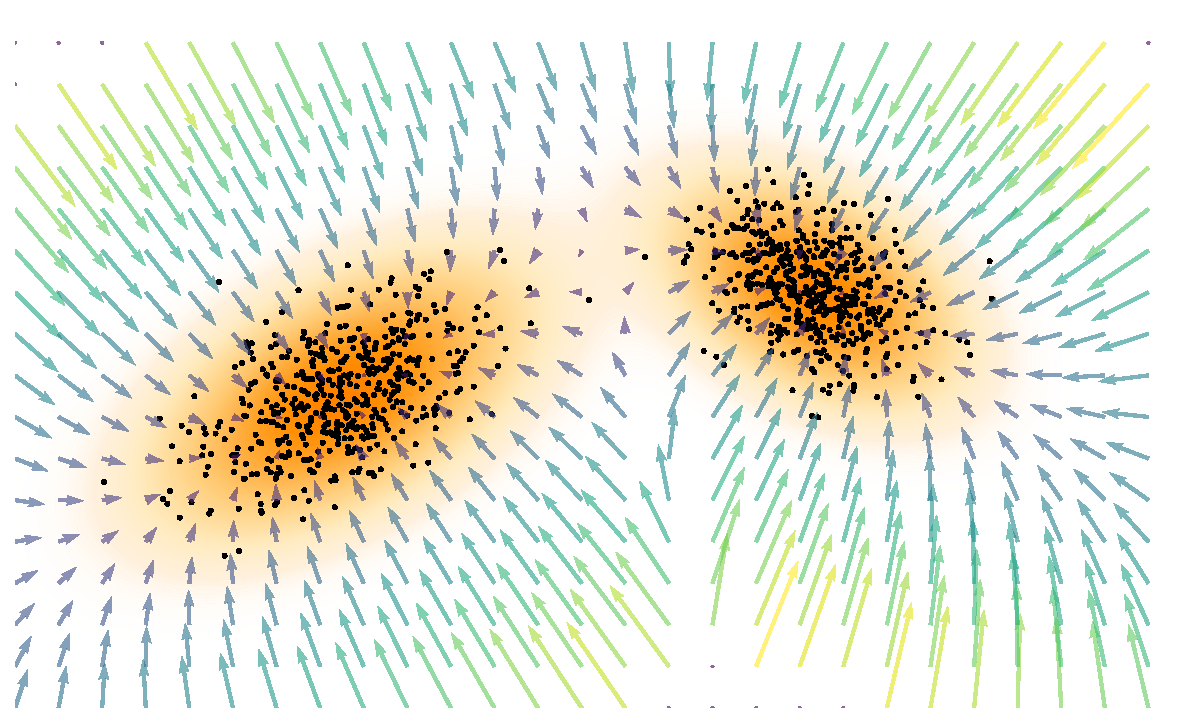
\includegraphics[width=0.95\linewidth]{Images/PartB/score_function_plot.pdf}
%     \caption{Visualization of score vector fields $\nabla_{\rvx} \log p(\rvx)$, which indicate the direction of increasing probability density under $p(\rvx)$.}
%     \label{fig:score-function}
% \end{figure}

% \paragraph{Why the Score Function Excels?}
% \jcr{A natural question arises: why model the score function instead of the probability distribution directly?
% The score provides both theoretical clarity and practical benefits. We start by outlining its conceptual foundations and will highlight further advantages as the chapter unfolds.}
% % One may question the rationale behind modeling the score function rather than the probability distribution itself.
% % \se{fix language. also transition to this paragraph is very rough, this was not mentioned before}
% % Indeed, the score function offers both theoretical and practical advantages. We begin by introducing its conceptual foundations and will progressively highlight additional benefits throughout this chapter.

% \subparagraph{1. Freedom from Normalization Constants.}
% Many distributions are defined only up to an unnormalized density $\tilde{p}(\rvx)$, e.g., $\exp(-E_{\bm{\phi}}(\rvx))$ in EBMs with
% \[
% p(\rvx) = \frac{\tilde{p}(\rvx)}{Z}, 
% \qquad 
% Z = \int \tilde{p}(\rvx)  \diff\rvx.
% \]
% Evaluating $Z_{\bm{\phi}}$ is generally intractable, creating a bottleneck for training.  
% The score function removes this difficulty:
% \begin{align}\label{eq:score-no-constant}
%     \nabla_{\rvx}\log p(\rvx) 
% = \nabla_{\rvx}\log \tilde{p}(\rvx) - \underbrace{\nabla_{\rvx}\log Z}_{=0}
% = \nabla_{\rvx}\log \tilde{p}(\rvx),
% \end{align}
% since $Z$ is constant in $\rvx$.  
% Hence the score depends only on $\tilde{p}$, allowing EBMs to be trained without computing $Z$.



% \subparagraph{2. A Complete and Expressive Representation.}
% Focusing on the score function does not entail any loss of information about the original distribution. The score function uniquely characterizes the distribution since it is the gradient of the log-density. Conversely, the original density can be recovered from the score function up to a constant:
% \[
% \log p(\rvx) = \log p(\rvx_0) + \int_0^1 \rvs(\rvx_0 + t(\rvx - \rvx_0))^\top (\rvx - \rvx_0)  \diff t,
% \]
% where $\rvx_0$ is a reference point and $\log p(\rvx_0)$ acts as an integration constant fixed by normalization. This equivalence establishes that modeling the score function is as expressive as modeling the density itself, offering a tractable alternative for generative modeling.




% \subsection{Training EBMs with Score Matching}\label{subsec:training-ebm}
% % \paragraph{Contrastive Divergence.} 
% % \se{should we cut this? not sure it's relevant}
% % One challenge in training EBMs is the difficulty of sampling from the model. A widely used workaround is \textit{Contrastive Divergence}, which approximates model samples using short-run MCMC.

% % We revisit \Cref{eq:mle-ebm}. Taking the gradient of the MLE objective with respect to $\bm{\phi}$ yields:
% % \begin{align*}
% %     &\nabla_{\bm{\phi}} \mathcal{L}_{\text{MLE}}(\bm{\phi}) \\
% %     =&\mathbb{E}_{p_{\text{data}}(\mathbf{x})} [-\nabla_{\bm{\phi}}E_{\bm{\phi}}(\rvx)] - \mathbb{E}_{p_{{\bm{\phi}}}(\mathbf{x})} [\nabla_{\bm{\phi}}\log Z_\bphi]\\
% %     =&\mathbb{E}_{p_{\text{data}}(\mathbf{x})} [-\nabla_{\bm{\phi}}E_{\bm{\phi}}(\rvx)] - \mathbb{E}_{p_{{\bm{\phi}}}(\mathbf{x})} \left[\frac{1}{Z_\bphi} \int \nabla_{\bm{\phi}} \exp(-E_{\bm{\phi}}(\rvx))    \diff\mathbf{x}\right]\\
% % = &\mathbb{E}_{p_{\text{data}}(\mathbf{x})} \left[ -\nabla_{\bm{\phi}} E_{\bm{\phi}}(\rvx) \right]
% % + \mathbb{E}_{p_{\bm{\phi}}(\mathbf{x})} \left[ \nabla_{\bm{\phi}} E_{\bm{\phi}}(\rvx) \right].
% % \end{align*}
% % This motivates the CD loss:
% % \begin{align}\label{eq:contrastive-div}
% %     \mathcal{L}_{\text{CD}}({\bm{\phi}}) 
% % = \mathbb{E}_{p_{\text{data}}(\mathbf{x})} [E_{\bm{\phi}}(\rvx)] 
% % - \mathbb{E}_{\tilde{p}_{{\bm{\phi}}}(\mathbf{x})} [E_{\bm{\phi}}(\rvx)],
% % \end{align}
% % where $\tilde{p}_{\bm{\phi}}(\mathbf{x})$ is an approximate distribution obtained by running a few MCMC steps (e.g., Langevin dynamics) initialized from a data point. This objective approximates the MLE gradient without requiring full convergence of the Markov chain. However, it still incurs computational cost due to the need to simulate MCMC at each training step.

% Maximum likelihood training of EBMs is difficult because of the partition function. 
% \emph{Score matching}~\citep{hyvarinen2005estimation} provides a practical alternative: rather than fitting normalized probabilities, 
% it aligns the score of the model with those of the data.  
% Since these gradients depend only on the energy function, score matching completely bypasses the partition function as we showed in \Cref{eq:score-no-constant}:
% \jcr{
% \begin{align*}
%     \nabla_{\mathbf{x}} \log p_{\bm{\phi}}(\mathbf{x}) &= \nabla_{\mathbf{x}} \log \frac{\exp(-E_{\bm{\phi}}(\rvx))}{Z_\bphi} \\ &= - \nabla_{\mathbf{x}} E_{\bm{\phi}}(\mathbf{x}) - \underbrace{\nabla_{\mathbf{x}} \log Z_\bphi}_{=0} \\&= - \nabla_{\mathbf{x}} E_{\bm{\phi}}(\mathbf{x}) ,
% \end{align*}
% }
% The score matching objective minimizes the discrepancy between the model's score and the (unknown) data score:
% \begin{align}\label{eq:ebm-sm}
% \mathcal{L}_{\mathrm{SM}}(\bm{\phi}) := \mathbb{E}_{p_{\mathrm{data}}(\mathbf{x})} \left[ \frac{1}{2} \left\| \nabla_{\mathbf{x}} \log p_{\bm{\phi}}(\mathbf{x}) - \nabla_{\mathbf{x}} \log p_{\mathrm{data}}(\mathbf{x}) \right\|_2^2 \right].
% \end{align}
% \paragraph{Score Matching: An Alternative Objective.}
% When the true data score $\nabla_{\mathbf{x}} \log p_{\mathrm{data}}(\mathbf{x})$ is inaccessible, score matching offers an ingenious alternative. Under mild regularity conditions (e.g., vanishing boundary terms), its objective can be elegantly reformulated using integration by parts (see Proposition~\ref{sm-trace}):
% \begin{align*}
% \mathcal{L}_{\mathrm{SM}}(\bm{\phi})
% = \mathbb{E}_{p_{\mathrm{data}}(\mathbf{x})} \left[
% \Tr\left(\nabla_{\mathbf{x}}^2 E_{\bm{\phi}}(\rvx) \right)
% + \frac{1}{2} \left\| \nabla_{\mathbf{x}} E_{\bm{\phi}}(\rvx) \right\|_2^2
% \right] + C,
% \end{align*}
% where $\nabla_{\mathbf{x}}^2 E_{\bm{\phi}}(\rvx)$ denotes the Hessian of $E_{\bm{\phi}}$ with respect to $\mathbf{x}$, and $C$ is a constant independent of $\bm{\phi}$.
% This formulation is particularly appealing because it removes the need to compute the intractable partition function $Z_\bphi$ and avoids costly sampling from the model distribution during training. Nevertheless, score matching introduces its own challenges. Specifically, the requirement to compute second-order derivatives (Hessians) often becomes computationally prohibitive, especially in high-dimensional settings.


\subsection{Motivation: What Is the Score?}\label{subsec:motivation-score}

For a density $p(\rvx)$ on $\mathbb{R}^D$, the \emph{score function} is the gradient of the log-density:
\[
\rvs(\rvx) := \nabla_{\rvx} \log p(\rvx), \qquad \rvs \colon \mathbb{R}^D \to \mathbb{R}^D.
\]
Intuitively, the score forms a vector field that points toward regions of higher probability, providing a local guide to where the data is most likely to occur (see \Cref{fig:score-function}).

\begin{figure}[th]
    \centering
    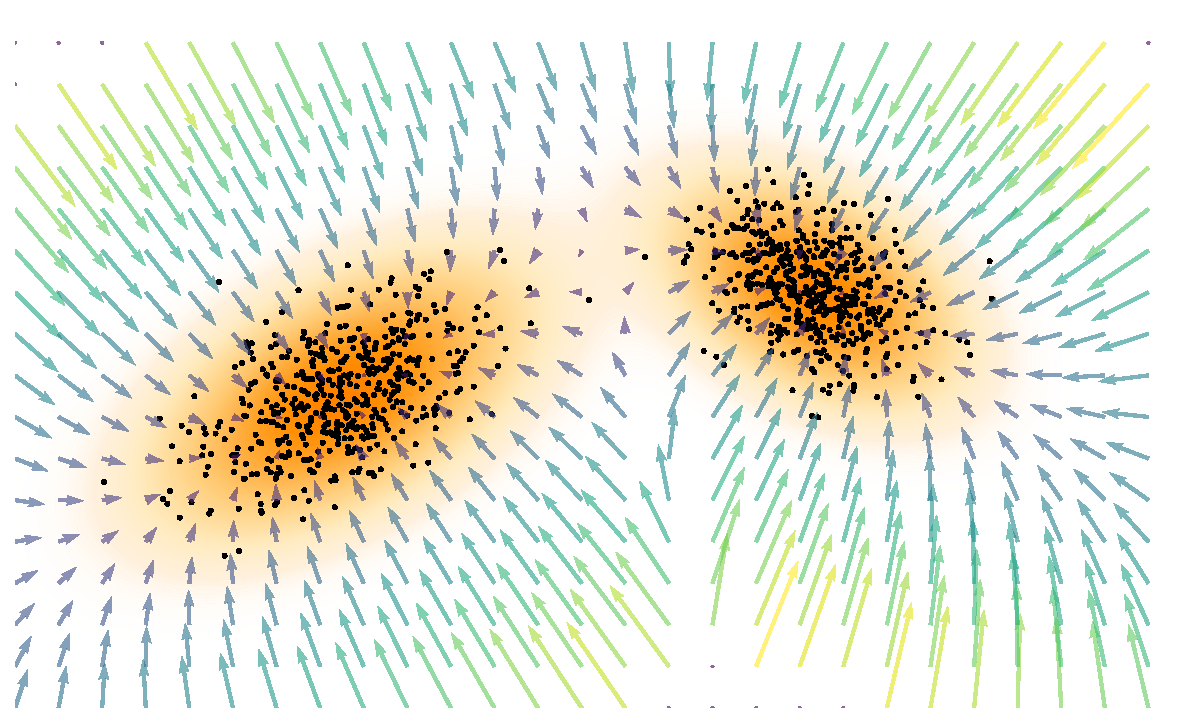
\includegraphics[width=0.95\linewidth]{Images/PartB/score_function_plot.pdf}
    \caption{\textbfs{Illustration of score vector fields.} Score vector fields $\nabla_{\rvx} \log p(\rvx)$ indicate directions of increasing density. \figcredit{Created by the authors.}}
    \label{fig:score-function}
\end{figure}

\paragraph{Why Model Scores Instead of Densities?}
Modeling the score offers both theoretical and practical benefits:


\subparagraph{1. Freedom from Normalization Constants.}  
    Many distributions are defined only up to an unnormalized density $\tilde{p}(\rvx)$, e.g., $\exp(-E_{\bm{\phi}}(\rvx))$ in EBMs:
    \[
    p(\rvx) = \frac{\tilde{p}(\rvx)}{Z}, 
    \qquad 
    Z = \int \tilde{p}(\rvx)\diff\rvx.
    \]
    While computing $Z$ is intractable, the score depends only on $\tilde{p}$:
\begin{align}\label{eq:score-compute}
\nabla_{\rvx}\log p(\rvx) = \nabla_{\rvx}\log \tilde{p}(\rvx) - \underbrace{\nabla_{\rvx}\log Z}_{=0} = \nabla_{\rvx}\log \tilde{p}(\rvx), \end{align} 
since $Z$ is constant in $\rvx$. This bypasses the partition function entirely.

\subparagraph{2. A Complete Representation.}  
The score function fully characterizes the underlying distribution.  
Since it is the gradient of the log-density, the density can be recovered (up to a constant) via
\[
\log p(\rvx) 
= \log p(\rvx_0) + \int_0^1 \rvs(\rvx_0 + t(\rvx - \rvx_0))^\top (\rvx - \rvx_0)  \diff t,
\]
where $\rvx_0$ is a reference point and $\log p(\rvx_0)$ is fixed by normalization.  
Thus, modeling the score is as expressive as modeling $p(\rvx)$ itself, while often more tractable for generative modeling.


\subsection{Training EBMs via Score Matching}\label{subsec:training-ebm}
In EBMs, the density is defined as $p_{{\bm{\phi}}}(\mathbf{x}) = \tfrac{\exp(-E_{\bm{\phi}}(\mathbf{x}))}{Z_\bphi}$. Maximum likelihood training requires computing $Z_{\bm{\phi}}$, which is generally intractable.  
A key observation is that the model score of $p_{{\bm{\phi}}}$ simplifies to: $-\nabla_{\rvx}E_{\bm{\phi}}(\rvx)$, independent of $Z_{\bm{\phi}}$ (see \Cref{eq:score-compute}).  

\emph{Score matching}~\citep{hyvarinen2005estimation} leverages the fact that scores depend only on the energy function.  
Instead of fitting normalized probabilities, it trains EBMs by aligning the model score with the (unknown) data score:
\begin{align}\label{eq:ebm-sm}
    \mathcal{L}_{\mathrm{SM}}(\bm{\phi}) 
= \tfrac{1}{2}  \mathbb{E}_{p_{\mathrm{data}}(\mathbf{x})} 
\big\| \nabla_{\mathbf{x}} \log p_{\bm{\phi}}(\mathbf{x}) 
- \nabla_{\mathbf{x}} \log p_{\mathrm{data}}(\mathbf{x}) \big\|_2^2.
\end{align}

Although the data score is inaccessible, integration by parts yields an equivalent expression involving only the energy and its derivatives (see Proposition~\ref{sm-trace} for more details):
\[
\mathcal{L}_{\mathrm{SM}}(\bm{\phi}) =
\mathbb{E}_{p_{\mathrm{data}}(\mathbf{x})} \left[
-\Tr \big(\nabla_{\mathbf{x}}^2 E_{\bm{\phi}}(\rvx)\big)
+ \tfrac{1}{2}  \|\nabla_{\mathbf{x}} E_{\bm{\phi}}(\rvx)\|_2^2
\right] + C,
\]
where $\nabla_{\mathbf{x}}^2 E_{\bm{\phi}}(\rvx)$ is the Hessian of $E_{\bm{\phi}}$ and $C$ is a constant independent of $\bm{\phi}$.  

This formulation is attractive because it eliminates the partition function and avoids sampling from the model during training.  
Its main drawback is the need for second-order derivatives: although one only needs the trace of the Hessian ($\Tr \big(\nabla_{\mathbf{x}}^2 E_{\bm{\phi}}\big)$), rather than the full Hessian matrix, exact computation of this term generally requires aggregating second-derivative information across input coordinates, so its cost typically increases with the input dimension $D$.  
We will revisit approaches to addressing this limitation later in the chapter.






\subsection{Langevin Sampling with Score Functions}\label{subsec:sampling-ebm}
Sampling from EBMs, defined by the energy function $E_{\bm{\phi}}(\mathbf{x})$, can be performed using \emph{Langevin dynamics}. We first present the discrete-time Langevin update and then its continuous-time limit as a stochastic differential equation (SDE). Finally, we discuss the physical intuition behind how Langevin dynamics enables efficient exploration of complex energy landscapes.


\begin{figure}
    \centering
    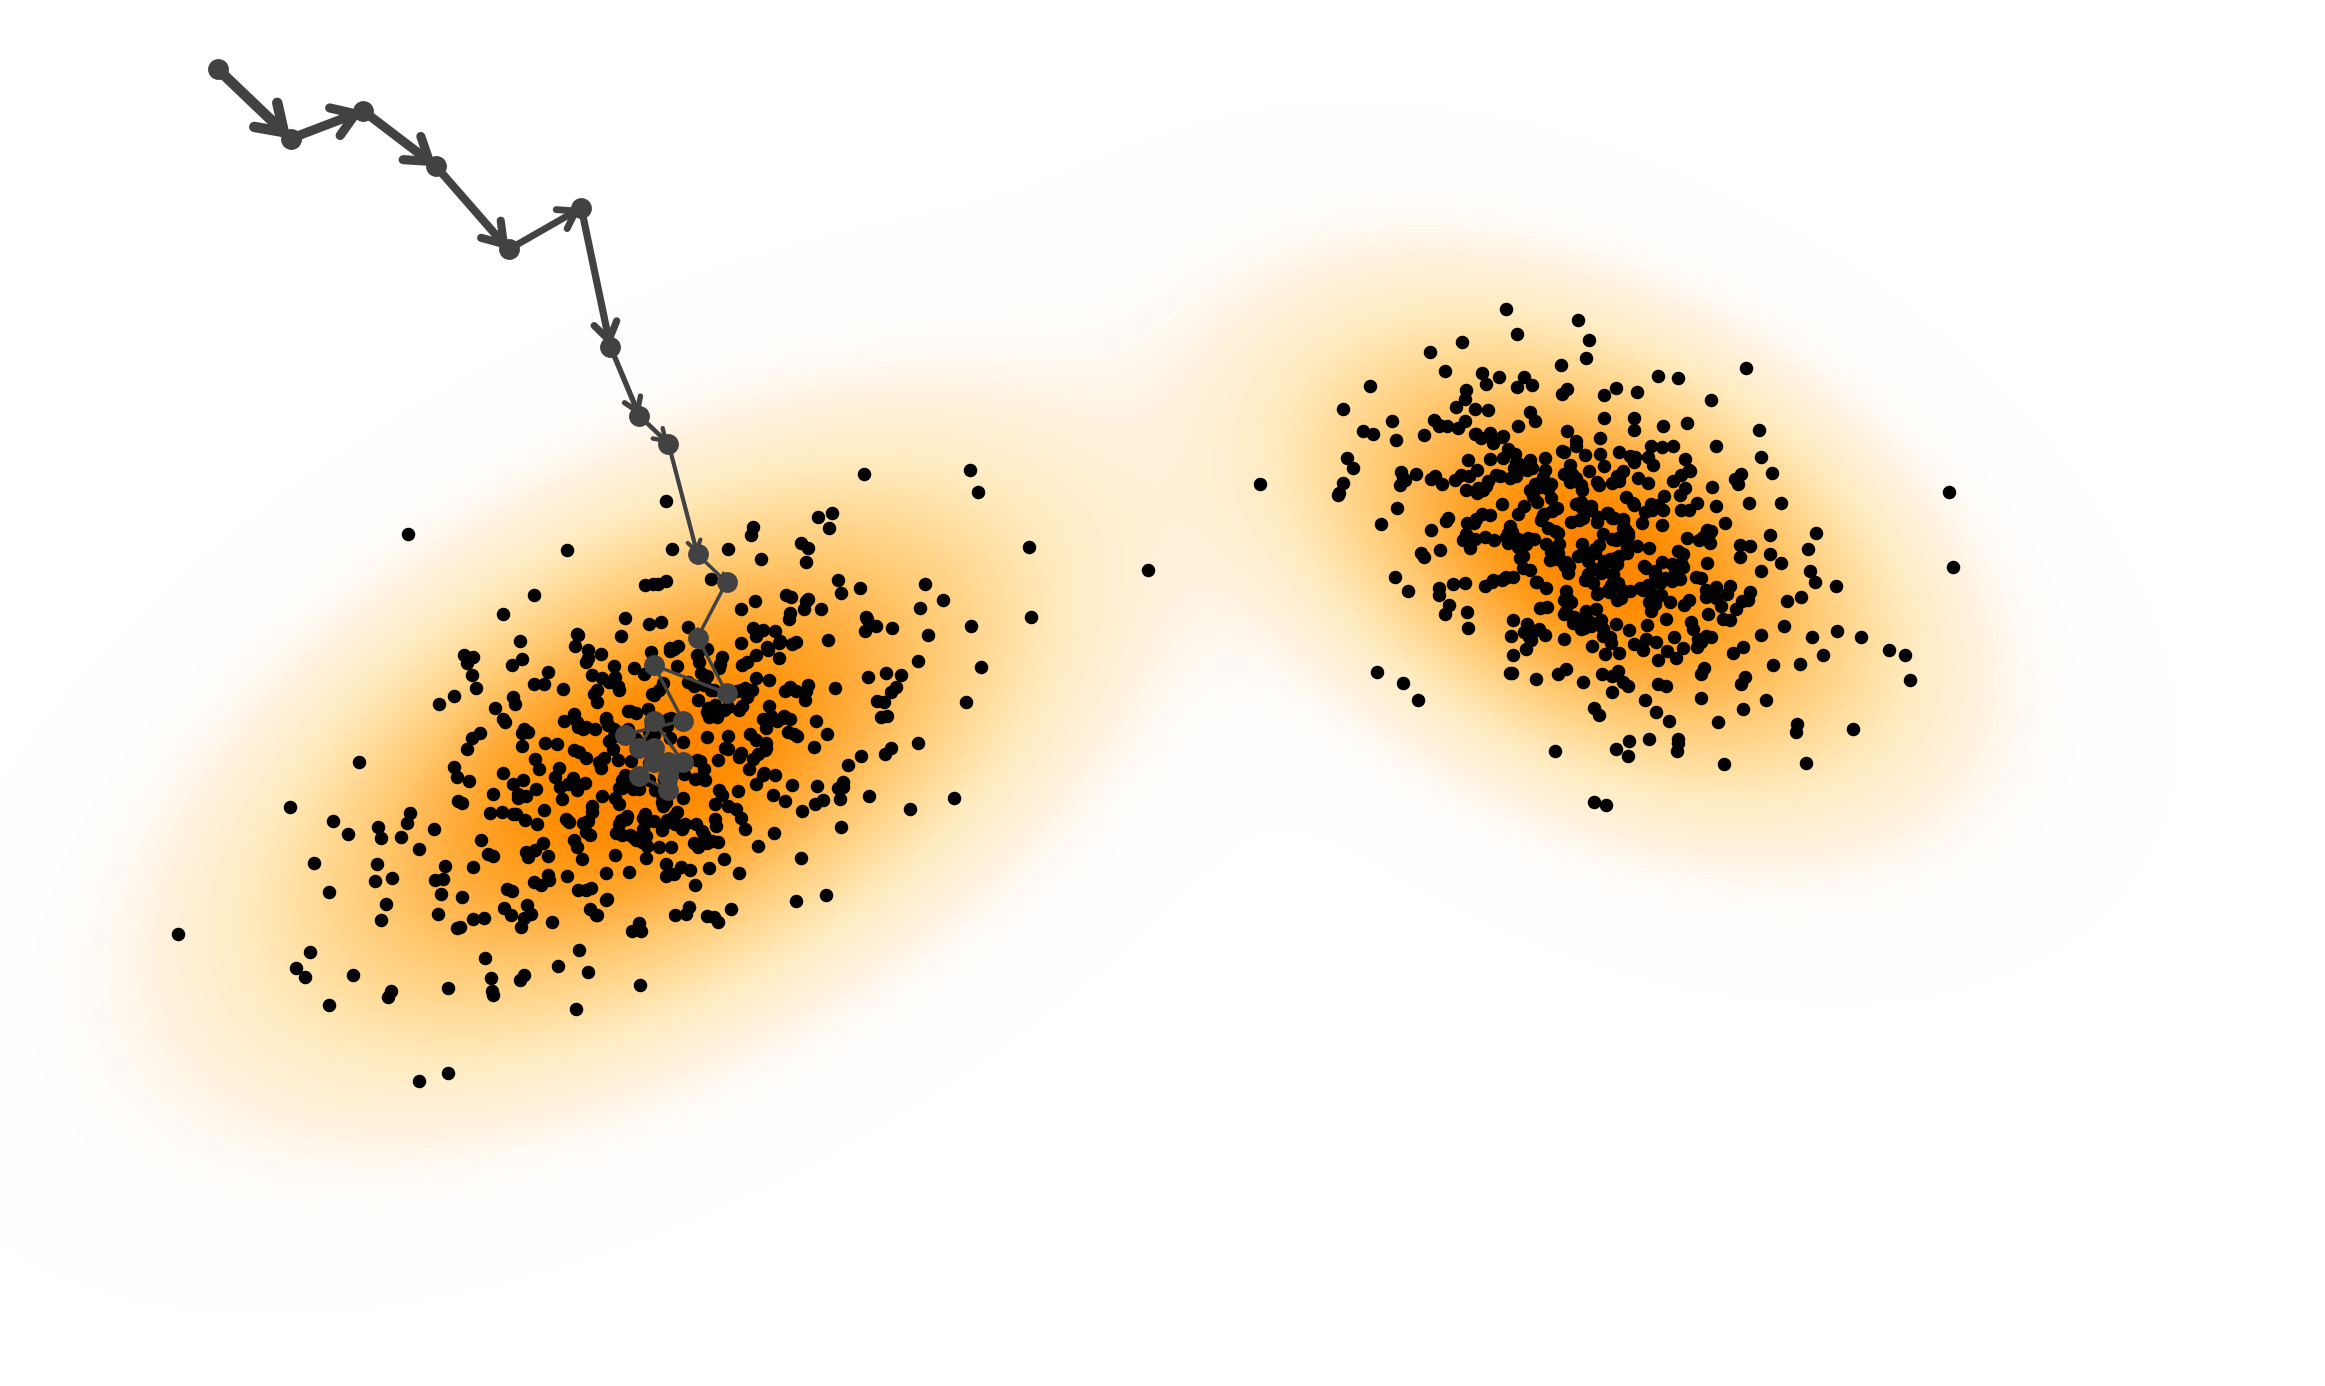
\includegraphics[width=\linewidth]{Images/PartB/langevin_sampling.png}
    \vspace{-1.5cm}
    \caption{\textbfs{Illustration of Langevin sampling.} Langevin sampling using the score function $\nabla_{\mathbf{x}} \log p_{\bm{\phi}}(\mathbf{x})$ to guide trajectories toward high-density regions via the update in \Cref{eq:discrete-langevin-score} (indicating by arrows). \figcredit{Created by the authors.}}
    \label{fig:langevin}
\end{figure}


\paragraph{Discrete-Time Langevin Dynamics.}
The discrete-time Langevin update is
\begin{align}\label{eq:discrete-langevin}
    \mathbf{x}_{n+1} = \mathbf{x}_n - \eta \nabla_{\mathbf{x}} E_{\bm{\phi}}(\mathbf{x}_n) +  \sqrt{2 \eta} \bm{\epsilon}_n, \quad n=0,1,2,\ldots,
\end{align}
where $\mathbf{x}_0$ is initialized from some distribution (often Gaussian), $\eta > 0$ is the step size, and $\bm{\epsilon}_n \sim \mathcal{N}(\mathbf{0}, \mathbf{I})$ is Gaussian noise. The noise enables exploration beyond local minima by adding stochasticity. 

Since the score function can be computed as 
\[
\nabla_{\mathbf{x}} \log p_{\bm{\phi}}(\mathbf{x}) = -\nabla_{\mathbf{x}} E_{\bm{\phi}}(\rvx).
\]
% \se{important to show why partition function disappears}
the update can equivalently be written as
\begin{align}\label{eq:discrete-langevin-score}
    \mathbf{x}_{n+1} = \mathbf{x}_n + \eta \nabla_{\mathbf{x}} \log p_{\bm{\phi}}(\mathbf{x}_n) + \sqrt{2 \eta}\bm{\epsilon}_n,
\end{align}
where the score function guides the samples toward high-density regions. This formulation is central to diffusion models, as will be detailed later.

\paragraph{Continuous-Time Langevin Dynamics.}
As the step size $\eta$ approaches zero, the discrete Langevin updates naturally converge to a continuous-time process described by the \emph{Langevin Stochastic Differential Equation (SDE)}\footnote{
With the factor $\sqrt{2}$, the Langevin dynamics leave $p_{\bm\phi}$ unchanged in time. Namely, $p_{\bm\phi}$ is stationary: if $\rvx(0)\sim p_{\bm\phi}$ then $\rvx(t)\sim p_{\bm\phi}$ for all $t\ge 0$. Equivalently, $p_{\bm\phi}$ is the stationary solution of the Fokker–Planck equation (see \Cref{app:continuity}):
\[
\partial_t \rho = -\nabla \cdot(\rho  \nabla\log p_{\bm\phi}) + \tfrac{\sigma^2}{2}\Delta \rho.
\]
Setting $\rho=p_{\bm\phi}$ gives $(\tfrac{\sigma^2}{2}-1)\Delta p_{\bm\phi}=0$, which holds only if $\sigma=\sqrt{2}$.
}
:
\begin{align}\label{eq:continuous-langevin}
 \diff \mathbf{x}(t) = \nabla_{\mathbf{x}} \log p_{\bm{\phi}}(\mathbf{x}(t)) \diff t + \sqrt{2} \diff \mathbf{w}(t),
\end{align}
where $\mathbf{w}(t)$ denotes a standard Brownian motion (also known as a Wiener process\footnote{Brownian increments satisfy
$\mathbf{w}(t+\eta)-\mathbf{w}(t)\sim \mathcal{N}(\mathbf{0},  \eta  \mathbf{I})$.
Euler–Maruyama therefore uses a step noise $\sqrt{2}  [\mathbf{w}(t+\eta)-\mathbf{w}(t)]
= \sqrt{2\eta}  \bm{\epsilon}_n$ with $\bm{\epsilon}_n \sim \mathcal{N}(\mathbf{0},\mathbf{I})$,
which explains the $\sqrt{\eta}$ factor.; this is the source of the square-root scaling. For a detailed introduction to Brownian motion and SDEs, please refer to \Cref{app:de}.}). It is important to understand that the discrete update rule in \Cref{eq:discrete-langevin} serves as the Euler–Maruyama discretization of this continuous SDE.
% \se{will people be confused by the square root on the step size?}


Under standard regularity assumptions (e.g., $p_{\bm{\phi}}\propto e^{-E_{\bm{\phi}}}$ with a confining, sufficiently smooth $E_{\bm{\phi}}$), the distribution of $\mathbf{x}(t)$ converges (exponentially fast) to $p_{\bm{\phi}}$ as $t\to\infty$; thus we can sample by simulating (solving) the SDE \Cref{eq:continuous-langevin}. 



\paragraph{Why Langevin Sampling?}
A natural way to understand Langevin sampling is through the lens of physics, where the energy function $ E_{\bm{\phi}}(\mathbf{x}) $ defines a potential landscape that shapes the behavior of particles. According to Newtonian dynamics, the motion of a particle under the force field derived from this energy is described by the ordinary differential equation (ODE)
\[
\diff \mathbf{x}(t) = -\nabla_{\mathbf{x}} E_{\bm{\phi}}\big(\mathbf{x}(t)\big)  \diff t,
\]
which deterministically drives the particle downhill toward a local minimum of the energy function. However, such deterministic dynamics can become trapped in local minima, preventing exploration of the full data distribution.

To overcome this limitation, Langevin dynamics introduces stochastic perturbations, resulting in the SDE
\[
\diff \mathbf{x}(t) = -\nabla_{\mathbf{x}} E_{\bm{\phi}}\big(\mathbf{x}(t)\big)  \diff t + \underbrace{\sqrt{2 } \diff \rvw(t)}_{\text{injected noise}},
\]
where $\rvw(t)$ is a standard Brownian motion. 
% and $\eta > 0$ is the diffusion coefficient controlling the noise intensity. \se{no diffusion coeff in equation}
The noise term allows the particle to escape local minima by crossing energy barriers, making the trajectory a stochastic process whose stationary distribution converges to the Boltzmann distribution
\[
p_{\bm{\phi}}(\mathbf{x}) \propto e^{-E_{\bm{\phi}}(\mathbf{x})}.
\]

From this perspective, EBMs can be viewed as learning a force field that pushes samples toward regions of high probability. Langevin sampling is particularly useful for EBMs because it provides a practical method to generate samples from the model distribution $p_{\bm{\phi}}(\mathbf{x})$ without explicitly computing the partition function. By iteratively applying the Langevin update, one obtains samples that approximate the target distribution.


\paragraph{Inherent Challenges of Langevin Sampling.}
Langevin dynamics, a widely used MCMC-based sampler, faces serious limitations in high-dimensional spaces. Its efficiency is highly sensitive to the choice of step size $\eta$, noise scale, and the number of iterations required to approximate the target distribution accurately. 

At the heart of this inefficiency lies the issue of poor ``mixing time'': In complex data distributions with many isolated modes, Langevin sampling often requires an extremely long time to transition between regions of high probability. This problem becomes significantly worse as dimensionality increases, leading to prohibitively slow convergence.

One can think of sampling as exploring a vast and rugged landscape with many distant valleys, each corresponding to a different data mode. Langevin dynamics, relying on local stochastic updates, struggles to traverse between these valleys efficiently. As a result, it often fails to capture the full diversity of the distribution.

This inefficiency hints the need for more structured and guided sampling methods that can navigate complex data manifolds more effectively than purely random exploration.



% Secondly, and also fundamentally, score matching primarily constrains the energy function only at the (local) training data points. It fails to impose explicit global regularization on the overall energy landscape, leaving energy values in regions far from training data loosely controlled. This can lead to undesirable or unconstrained model behavior, a crucial difference from directly modeling probability densities. The latter inherently regularizes the entire distribution by implicitly enforcing a global ``sum-to-one'' rule on probabilities, ensuring more stable energy values across the data space.
% \subsection{Closing Remark}
% EBMs and score matching are closely connected. While much research has focused on improving the efficiency and scalability of score matching for training EBMs~\citep{vincent2011connection,song2020sliced}, its role has significantly evolved. Originally developed as an elegant solution to the intractable normalization constant in unnormalized statistical models such as EBMs, score matching has since become a fundamental building block of modern diffusion models. We will explore this important connection in greater detail in the following sections.






\clearpage
\newpage

% \se{the structure of this chapter is unecessarily convoluted. the story is going to be cleaner if you don't mark the background as optional (anyways it's short) and have a coherent story where you have representation, learning, inference. right now therre is too much back and forth between scores, sampling, score matching}


% Consider a landscape representing the probability distribution over data points, where regions of higher elevation correspond to higher likelihoods, and lower regions correspond to lower likelihoods. At each point in this landscape, imagine an arrow indicating the direction of steepest ascent, guiding movement toward areas of increasing probability. This vector field is known as the \emph{score function}~\citep{stein1972bound}, providing an intuitive and precise direction for navigating the probability landscape.


% \subsection{Motivation--What Is Score?}
% We begin by formally defining the score function. For a probability density function $ p(\rvx) $ on $ \mathbb{R}^D $, the \emph{score function} is the vector field given by the gradient of the log-density:
% \[
% \rvs(\rvx) := \nabla_{\rvx} \log p(\rvx),
% \]
% where $ \rvs \colon \mathbb{R}^D \to \mathbb{R}^D $.

% \begin{figure}[th]
%     \centering
%     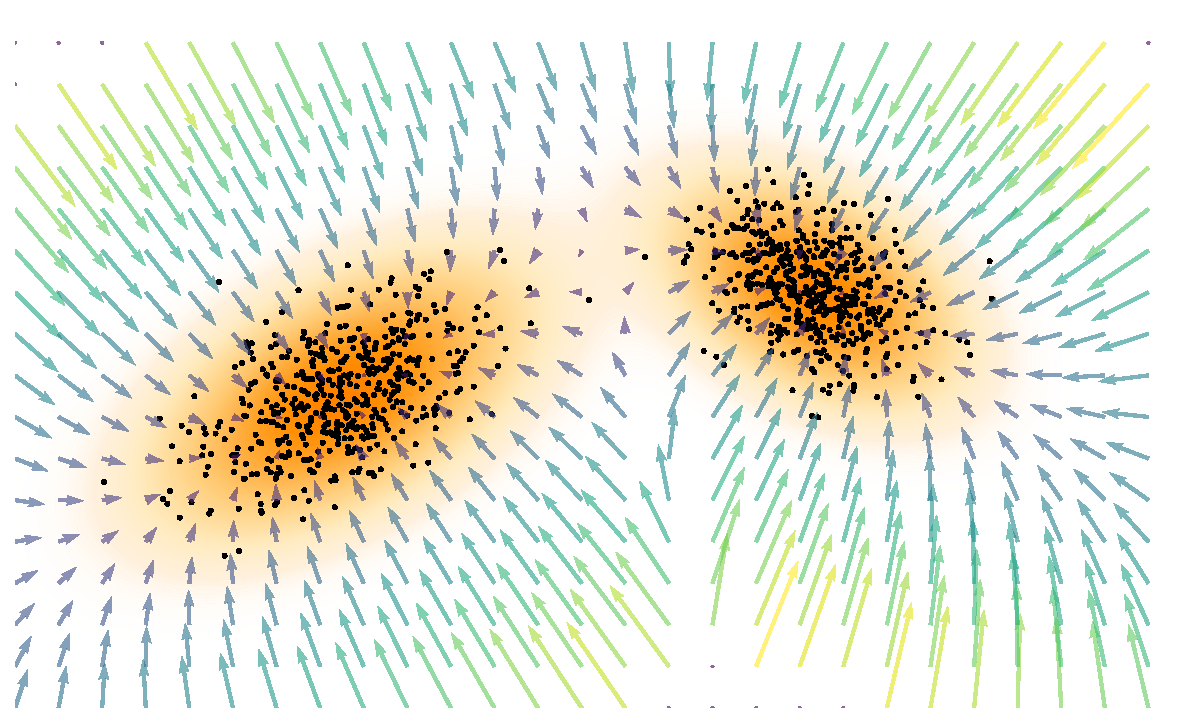
\includegraphics[width=0.95\linewidth]{Images/PartB/score_function_plot.pdf}
%     \caption{Visualization of score vector fields $\nabla_{\rvx} \log p(\rvx)$, which indicate the direction of increasing probability density under $p(\rvx)$.}
%     \label{fig:score-function}
% \end{figure}

% \paragraph{Why the Score Function Excels?}
% One may question the rationale behind modeling the score function rather than the probability distribution itself.
% \se{fix language. also transition to this paragraph is very rough, this was not mentioned before}
% Indeed, the score function offers both theoretical and practical advantages. We begin by introducing its conceptual foundations and will progressively highlight additional benefits throughout this chapter.

% \subparagraph{1. Freedom from Normalization Constants.}
% Many probability distributions are initially defined by an unnormalized density $\tilde{p}(\rvx)$. To turn this into a true probability density $ p(\rvx) $, we must divide by a normalization constant $Z = \int \tilde{p}(\rvx)    \diff \rvx$. Calculating this $Z$ is often computationally prohibitive, involving intractable integrals. This difficulty is a significant bottleneck in training many models, such as EBMs.

% The score function, however, elegantly bypasses this challenge. Consider the derivative:
% \[
% \nabla_{\rvx} \log p(\rvx) = \nabla_{\rvx} \log \left( \frac{\tilde{p}(\rvx)}{Z} \right) = \nabla_{\rvx} \log \tilde{p}(\rvx) - \underbrace{\nabla_{\rvx} \log Z}_{=0}.
% \]
% Since $Z$ is a constant with respect to $ \rvx $, its gradient is zero.
% \[
% \nabla_{\rvx} \log p(\rvx) = \nabla_{\rvx} \log \tilde{p}(\rvx).
% \]
% This remarkable property means the score function is entirely independent of the normalization constant. We can operate directly with unnormalized densities, freeing us from the immense computational burden of computing or approximating $Z$.

% \subparagraph{2. A Complete and Expressive Representation.}
% Focusing on the score function does not entail any loss of information about the original distribution. The score function uniquely characterizes the distribution since it is the gradient of the log-density. Conversely, the original density can be recovered from the score function up to a constant:
% \[
% \log p(\rvx) = \log p(\rvx_0) + \int_0^1 \rvs(\rvx_0 + t(\rvx - \rvx_0))^\top (\rvx - \rvx_0)  \diff t,
% \]
% where $\rvx_0$ is a reference point and $\log p(\rvx_0)$ acts as an integration constant fixed by normalization. This equivalence establishes that modeling the score function is as expressive as modeling the density itself, offering a tractable alternative for generative modeling.



% \paragraph{Using the Score for Generation.}
% Having established that the score function  is a complete and unburdened representation of a distribution, a pivotal question arises:
% \begin{question}
%     Can we actually generate new samples from a complex data distribution if we only know its score function, $ \rvs(\cdot) = \nabla_{\rvx} \log p_{\mathrm{data}}(\cdot) $?
% \end{question}
% The answer is affirmative, owing to a powerful iterative procedure,  \emph{Langevin dynamics}, as introduced in \Cref{eq:discrete-langevin-score}:
% \begin{align}\label{eq:score-langevin}
%     \rvx_{n+1} = \rvx_n + \eta \rvs(\rvx_n) + \sqrt{2\eta} \bm{\epsilon}_n, \quad n=0,1,2,\dots,
% \end{align}
% The process begins from an arbitrary initial point $\rvx_0$ with a step size $\eta > 0$. At each iteration, the sample is nudged in the direction of the score,  ascending the probability landscape; while random noise encourages exploration. Under suitable conditions, \se{need to cite and probably say what the conditions are for completeness} this simple yet powerful procedure produces samples from $p_{\mathrm{data}}$. This demonstrates a key strength of score-based modeling: generating realistic data requires only the score function, not the full probability density.

\section{\texorpdfstring{From Energy-Based to Score-Based Generative Models}{From Energy-Based to Score-Based Generative Models}}
EBMs show that generation depends only on the score, which points toward regions of higher probability, rather than on the full normalized density. 
While score matching avoids the partition function, training through the energy still requires expensive second derivatives. 
The key idea is that since sampling with Langevin dynamics needs only the score, we can learn it directly with a neural network. 
This shift, from modeling energies to modeling scores, forms the foundation of score-based generative models.






\begin{figure}[ht!]
    \centering
    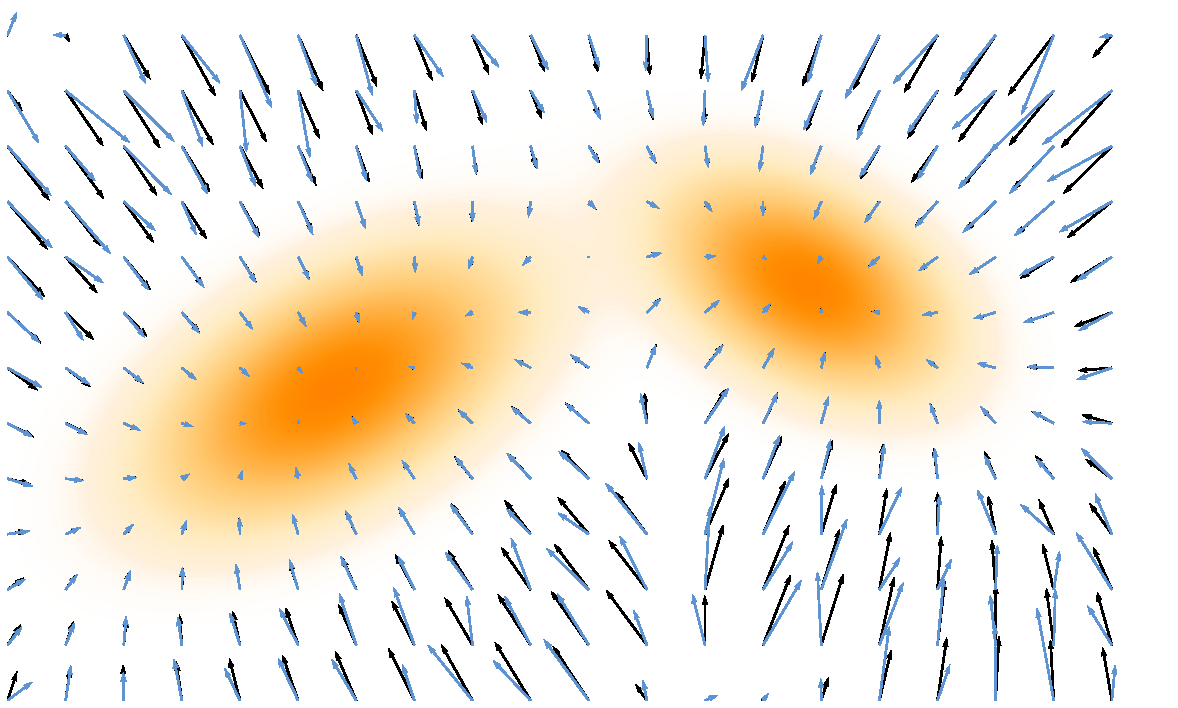
\includegraphics[width=0.9\linewidth]{Images/PartB/score_function_approximation.pdf}
    \caption{\textbfs{Illustration of Score Matching.} The neural network score ${\color{customblue}\rvs_{\bm{\phi}}(\rvx)}$ is trained to match the ground truth score $\rvs(\rvx)$ using a MSE loss. Both are represented as vector fields. \figcredit{Created by the authors.}}
    \label{fig:sm-illustration}
\end{figure}

\subsection{Training with Score Matching}\label{subsec:training-sm}
\paragraph{Score Matching.}
To approximate the score function $\rvs(\rvx) = \nabla_{\rvx} \log p_{\mathrm{data}}(\rvx)$ from samples of $p_{\mathrm{data}}$,  
we approximate it directly as a vector field parameterized by a neural network $\rvs_{\bm{\phi}}(\rvx)$ (see \Cref{fig:sm-illustration}):
\[
\rvs_{\bm{\phi}}(\rvx) \approx \rvs(\rvx).
\]
\emph{Score matching} fits this vector field by minimizing the mean squared error (MSE) between the true and estimated scores:
\begin{mdframed}
\begin{align}\label{eq:sm}
    \mathcal{L}_{\mathrm{SM}}(\bm{\phi}) 
    := \frac{1}{2}  \mathbb{E}_{\rvx \sim p_{\mathrm{data}}}
    \Big[\| \rvs_{\bm{\phi}}(\rvx) - \rvs(\rvx)\|_2^2\Big].
\end{align}
\end{mdframed}

\paragraph{Tractable Score Matching.}
At first glance, this objective seems infeasible because the true score $\rvs(\rvx)$, which serves as the regression target, is unknown.  
Fortunately, \citet{hyvarinen2005estimation} showed that integration by parts yields an equivalent objective that depends only on the model $\rvs_{\bm{\phi}}$ and the data samples, without requiring access to the true score.  
We state this key result in the following proposition: 
\proppp{Hyvärinen’s Tractable Form of SM}{sm-trace}
        {
        We can express the following equation as:
        \begin{align*}
            \mathcal{L}_{\text{SM}}(\bm{\phi}) = \widetilde{\mathcal{L}}_{\text{SM}}(\bm{\phi}) + C.
        \end{align*}
        where
        \begin{align}\label{eq:sm-alternative}
            \widetilde{\mathcal{L}}_{\text{SM}}(\bm{\phi})
            := \mathbb{E}_{\rvx \sim p_{\text{data}}(\rvx)} \left[
            \Tr\left(\nabla_{\rvx}\rvs_{\bm{\phi}}(\rvx)\right)
            + \frac{1}{2} \norm{\rvs_{\bm{\phi}}(\rvx)}_2^2
            \right].
        \end{align}
        and $C$ is a constant that does not depend on $\bm{\phi}$. The minimizer $\rvs^*$ is obtained as: $\rvs^*(\cdot) = \nabla_{\rvx} \log p(\cdot)$.
        }
        {The result follows by expanding the MSE in $ \mathcal{L}_{\text{SM}} $ and applying integration by parts. The proof is given in \Cref{app-sec:sm-trace}. 
        }

Using the equivalent objective in \Cref{eq:sm-alternative}, we train the score model $\rvs_{\bm{\phi}}(\rvx)$ solely from observed samples of $p_{\mathrm{data}}$, eliminating the need for the true score function.


\paragraph{Intuition of \Cref{eq:sm-alternative}.}
The alternative score matching objective $\widetilde{\mathcal{L}}_{\text{SM}}(\bm\phi)$
can be understood from its two terms.
The norm term $\tfrac12\|\rvs_{\bm\phi}(\rvx)\|^2$ penalizes large score values,
especially in regions where $p_{\mathrm{data}}$ is large.
The divergence term $\Tr(\nabla_{\rvx} \rvs_{\bm\phi}(\rvx))$ appears with a positive sign in the loss, so minimizing the objective also favors locally contracting behavior.
Together, these two terms yield the population-optimal score field
$\rvs^*(\rvx)=\nabla_{\rvx}\log p_{\mathrm{data}}(\rvx)$.
We explain the geometric intuition in more detail below.

\subparagraph{Effect of the Magnitude Term.}
Since the expectation in $\widetilde{\mathcal{L}}_{\mathrm{SM}}(\bm\phi)$ is taken under
$p_{\mathrm{data}}$, regions where $p_{\mathrm{data}}(\rvx)$ is large (high data density)
contribute more strongly to the loss. The magnitude term
$\tfrac12\|\rvs_{\bm\phi}(\rvx)\|^2$ therefore places a stronger penalty on large
score values in these regions. By itself, however, this term does not imply that
$\rvs_{\bm\phi}(\rvx)=\mathbf{0}$ at every high-density point; at the population
optimum,
\[
\rvs^*(\rvx)=\nabla_{\rvx}\log p_{\mathrm{data}}(\rvx),
\]
which vanishes only at stationary points of the log-density.

\subparagraph{Concavity When the Field is (Approximately) a Gradient.}
Because the divergence term $\Tr(\nabla_{\rvx} \rvs_{\bm\phi}(\rvx))$ enters the loss with a positive sign, minimizing the objective favors
negative divergence in regions emphasized by the data distribution.
Negative divergence indicates net local contraction, although by itself it does
not guarantee that a stationary point is a sink.
To make this precise, assume
$\rvs_{\bm\phi}=\nabla_{\rvx}u$ for a scalar function $u:\R^D\to\R$, as is natural when matching a
log density. Then $\nabla_{\rvx}\rvs_{\bm\phi}=\nabla_{\rvx}^2 u$ (the Hessian) and
$\nabla \cdot \rvs_{\bm\phi}(\rvx)=\Tr(\nabla_{\rvx}^2 u(\rvx))$ (the divergence).

At a stationary point $\rvx_\star$, where $\rvs_{\bm\phi}(\rvx_\star)=\nabla_{\rvx}u(\rvx_\star)=\mathbf{0}$,
a second order Taylor expansion gives
\[
u(\rvx)
= u(\rvx_\star)
+ \tfrac12(\rvx-\rvx_\star)^\top \nabla_{\rvx}^2 u(\rvx_\star)(\rvx-\rvx_\star)
+ o(\|\rvx-\rvx_\star\|^2).
\]
If the Hessian $\nabla_{\rvx}^2 u(\rvx_\star)$ is negative definite, then $u$ is locally concave at
$\rvx_\star$ and the log density attains a strict local maximum\footnote{We remark that strict concavity (and thus a strict local maximum of the log density) requires the entire Hessian
$\nabla_{\rvx}^2 u$ to be negative definite, not merely to have negative trace.
A negative trace guarantees that the sum of eigenvalues is negative, but some eigenvalues could still
be positive, leading to a saddle point rather than a maximum.
} there.
Because all eigenvalues of the Hessian are negative, the trace is also negative:
$\Tr(\nabla_{\rvx}^2 u(\rvx_\star))<0$.
Thus, in this case, the stationary point is locally attracting under the score field:
small perturbations are pulled back toward $\rvx_\star$.






\subsection{Sampling with Langevin Dynamics}
Once trained by minimizing \Cref{eq:sm-alternative}, the score model $\rvs_{\bm{\phi}^\times}(\rvx)$ can replace the oracle score in Langevin dynamics for sampling:
\begin{align}\label{eq:score-langevin-emp}
    \mathbf{x}_{n+1} = \mathbf{x}_n + \eta   \rvs_{\bm{\phi}^\times}(\rvx_n) + \sqrt{2\eta}    \bm{\epsilon}_n, \quad \bm{\epsilon}_n \sim \mathcal{N}(\bm{0}, \bm{I}),
\end{align}
for $n=0,1,2,\dots$, initialized at $\rvx_0$. As in the EBM case \Cref{eq:continuous-langevin}, this recursion is precisely the Euler–Maruyama discretization of the continuous-time Langevin SDE:
\begin{align*}
    \diff \rvx(t) = \rvs_{\bm{\phi}^\times}(\rvx(t)) \diff t + \sqrt{2} \diff \mathbf{w}(t),
\end{align*}
with initialization $\rvx(0)$. Hence, in the limit of small step size, the discrete and continuous formulations coincide.  In practice, one can either run the discrete sampler or directly simulate the SDE.



\subsection{Prologue: Score-Based Generative Models}

In the remainder of this chapter, we examine the foundational role of the score function in modern diffusion models. Initially introduced to enable efficient training of EBMs, the score function has evolved into a central component of a new generation of generative models. Building on this foundation, we explore how the score function informs the theoretical formulation and practical implementation of \emph{score-based diffusion models}, offering a principled framework for data generation via stochastic processes.


\clearpage
\newpage


\section{\texorpdfstring{Denoising Score Matching}{Denoising Score Matching}}\label{sec:dsm}

\subsection{Motivation}
Although the alternative objective in \Cref{eq:sm-alternative}
\begin{align*}
    \widetilde{\mathcal{L}}_{\text{SM}}(\bm{\phi}) = \mathbb{E}_{\rvx \sim p_{\mathrm{data}}} \left[\mathrm{Tr}\big(\nabla_{\rvx}\rvs_{\bm{\phi}}(\rvx)\big) + \frac{1}{2} \|\rvs_{\bm{\phi}}(\rvx)\|_2^2 \right]
\end{align*}
is more tractable, it still requires computing the trace of the Jacobian, $\mathrm{Tr}(\nabla_{\rvx}\rvs_{\bm{\phi}}(\rvx))$. Although this does not require forming the full Jacobian matrix, exact evaluation generally becomes more expensive as the input dimension $D$ increases, since it requires aggregating derivative information across input coordinates. This can therefore be computationally expensive in high dimensions.


To address this, sliced score matching~\citep{song2020sliced} replaces the trace term with a stochastic estimate based on random projections. We briefly outline the idea below.
% \se{perhaps mention huthcinson's trick since they are equivalent}
\paragraph{Sliced Score Matching and Hutchinson's Estimator.} Sliced score matching  replaces the trace in score matching by averaging directional derivatives along random ``slices''. Let $\rvu\in\R^D$ be an \emph{isotropic} random vector (e.g., Rademacher or standard Gaussian) with
$\E[\rvu]=0$ and $\E[\rvu\rvu^\top]=\mathbf I$. By Hutchinson’s identity 
\[
\Tr(\rmA)=\E_{\rvu}[\rvu^\top \rmA \rvu],\quad\text{and}\quad\E_{\rvu}[(\rvu^\top\rvs_{\bphi}(\rvx))^2]=\|\rvs_{\bphi}(\rvx)\|_2^2,
\]
 we obtain the exact form
\[
\widetilde{\mathcal{L}}_{\mathrm{SM}}(\bphi)
=\E_{\rvx,\rvu} \Big[\rvu^\top\big(\nabla_{\rvx}\rvs_{\bphi}(\rvx)\big)\rvu+\tfrac12(\rvu^\top\rvs_{\bphi}(\rvx))^2\Big].
\]
This objective can be evaluated efficiently with automatic differentiation, using Jacobian- and vector-Jacobian-product operations (JVP/VJP) instead of explicitly computing large Jacobian or Hessian matrices.
Averaging over $K$ random probes yields an unbiased estimator with variance $\mathcal{O}(1/K)$, 
and the directional term $\rvu^\top(\nabla_{\rvx}\rvs_{\bphi})\rvu$ can be computed 
efficiently using JVP/VJP routines without explicit Jacobians.  Intuitively, this means we only check the model’s behavior along random directions: 
the projected score is nudged to align with regions of higher data density, 
so data points become stationary in expectation. 

\paragraph{From Sliced to Denoising Score Matching.} Sliced score matching sidesteps Jacobians but still relies on the raw data distribution. 
This makes it fragile: for image data lying on low-dimensional manifolds, 
the score $\nabla_{\rvx}\log p_{\mathrm{data}}(\rvx)$ may be undefined or unstable, 
and the method only constrains the vector field at observed points, 
providing weak control in their neighborhoods. 
It further suffers from probe-induced variance and repeated JVP/VJP costs. 

A more robust alternative, which we focus on here, is \emph{Denoising Score Matching} (DSM)~\citep{vincent2011connection}, 
which offers a principled and scalable solution.



\subsection{Training}
Let us revisit the SM loss in \Cref{eq:sm}:
\begin{align*}
     \mathcal{L}_{\text{SM}}(\bm{\phi}) =  \frac{1}{2} \mathbb{E}_{\rvx \sim p_{\text{data}}(\rvx)} \left[ \norm{\rvs_{\bm{\phi}}(\rvx) - \nabla_{\rvx} \log p_{\text{data}}(\rvx)}_2^2 \right],
\end{align*}
where the issue arises from the intractable term $\nabla_{\rvx} \log p_{\text{data}}(\rvx)$.

\paragraph{\citet{vincent2011connection}'s Solution by Conditioning.}
To overcome the intractability of $\nabla_{\rvx} \log p_{\text{data}}(\rvx)$, \citet{vincent2011connection} proposed injecting noise into the data $\rvx \sim p_{\text{data}}$ via a known conditional distribution $p_{\sigma}(\tilde{\rvx}|\rvx)$ with scale $\sigma$. The neural network $\rvs_{\bm{\phi}}(\tilde{\rvx}, \sigma)$ is trained to approximate the score of the marginal perturbed distribution
\[
p_\sigma(\tilde{\rvx}) = \int p_{\sigma}(\tilde{\rvx}|\rvx) p_{\text{data}}(\rvx) \diff \rvx
\]
by minimizing the loss
\begin{align}\label{eq:sm-noise-loss}
\mathcal{L}_{\text{SM}}(\bm{\phi}; \sigma) := \frac{1}{2} \mathbb{E}_{\tilde{\rvx} \sim p_\sigma} \left[ \norm{\rvs_{\bm{\phi}}(\tilde{\rvx}, \sigma) - \nabla_{\tilde{\rvx}} \log p_\sigma(\tilde{\rvx})}_2^2 \right].
\end{align}

Even though $\nabla_{\tilde{\rvx}} \log p_\sigma(\tilde{\rvx})$ is generally intractable, \citet{vincent2011connection} showed that \emph{conditioning} on $\rvx \sim p_{\text{data}}$ yields an equivalent, tractable objective—the \emph{Denoising Score Matching} (DSM) loss:
\begin{mdframed}
\begin{align}\label{eq:dsm-loss}
\mathcal{L}_{\text{DSM}}(\bm{\phi}; \sigma) := \frac{1}{2} \mathbb{E}_{\rvx \sim p_{\text{data}}, \tilde{\rvx} \sim p_{\sigma}(\cdot|\rvx)} \left[ \norm{\rvs_{\bm{\phi}}(\tilde{\rvx}, \sigma) - \nabla_{\tilde{\rvx}} \log p_{\sigma}(\tilde{\rvx}|\rvx)}_2^2 \right].
\end{align}
\end{mdframed}

The optimal minimizer $\rvs^*$ of \Cref{eq:dsm-loss} satisfies
\[
\rvs^*(\tilde{\rvx}, \sigma) = \nabla_{\tilde{\rvx}} \log p_\sigma(\tilde{\rvx}),
\]
which is also optimal for \Cref{eq:sm-noise-loss}.

For example, when $p_{\sigma}(\tilde{\rvx}|\rvx)$ is Gaussian noise with variance $\sigma^2$,
\[
p_{\sigma}(\tilde{\rvx}|\rvx) = \mathcal{N}(\tilde{\rvx}; \rvx, \sigma^2 \mathbf{I}),
\]
the gradient $\nabla_{\tilde{\rvx}} \log p_{\sigma}(\tilde{\rvx}|\rvx)$ has a closed form (see \Cref{eq:gaussian-dsm}), making the regression target explicit and computationally tractable.

Moreover, as $\sigma \approx 0$, $p_\sigma(\tilde{\rvx}) \approx p_{\text{data}}(\rvx)$ and
\[
\rvs^*(\tilde{\rvx}, \sigma) = \nabla_{\tilde{\rvx}} \log p_\sigma(\tilde{\rvx}) \approx \nabla_{\rvx} \log p_{\text{data}}(\rvx),
\]
indicating the learned score approximates the original data score, enabling its use in generation.

We formalize this discussion on the gradient equivalence between $\mathcal{L}_{\text{SM}}$ and $\mathcal{L}_{\text{DSM}}$ in the following theorem:
\thmp{Equivalence of $\mathcal{L}_{\text{SM}}$ and $\mathcal{L}_{\text{DSM}}$}{sm-dsm}{
For any fixed noise scale $\sigma > 0$, the following holds:
\begin{align}\label{eq:score-matching}
    \mathcal{L}_{\text{SM}}(\bm{\phi}; \sigma) = \mathcal{L}_{\text{DSM}}(\bm{\phi}; \sigma) + C,
\end{align}
where $C$ is a constant independent of the parameter $\bm{\phi}$. Furthermore, the minimizer $\rvs^*(\cdot, \sigma)$ of both losses satisfies
\[
    \rvs^*(\tilde{\rvx}, \sigma) = \nabla_{\tilde{\rvx}} \log p_\sigma(\tilde{\rvx}), \quad \text{for almost every } \tilde{\rvx}.
\]
}{The equivalence follows from a direct computation: by expanding the MSE in $\mathcal{L}_{\text{SM}}$ and $\mathcal{L}_{\text{DSM}}$, all $\bm{\phi}$-dependent terms cancel, leaving only a constant difference independent of $\bm{\phi}$.\\
 The derivation of the minimizer follows the same argument as in Proposition~\ref{dsm-minimizer}. We defer the detailed derivation to \Cref{app-sec:sm-dsm}.
}

This theorem, like Theorem~\ref{thm:equiv-marginal-kl} in DDPM, illustrates a key shared principle:
\msg{Insight}{Conditioning Technique}{The conditioning technique also appears in the variational view of diffusion models in DDPM (see Theorem~\ref{thm:equiv-marginal-kl}), where conditioning on a data point $\rvx$ turns an intractable loss into a tractable one for Monte Carlo estimation. A similar idea arises in the flow-based perspective (e.g., Flow Matching~\citep{lipman2022flow}), as we will see in \Cref{sec:flow-matching-framework}.}


\begin{figure}
    \centering
    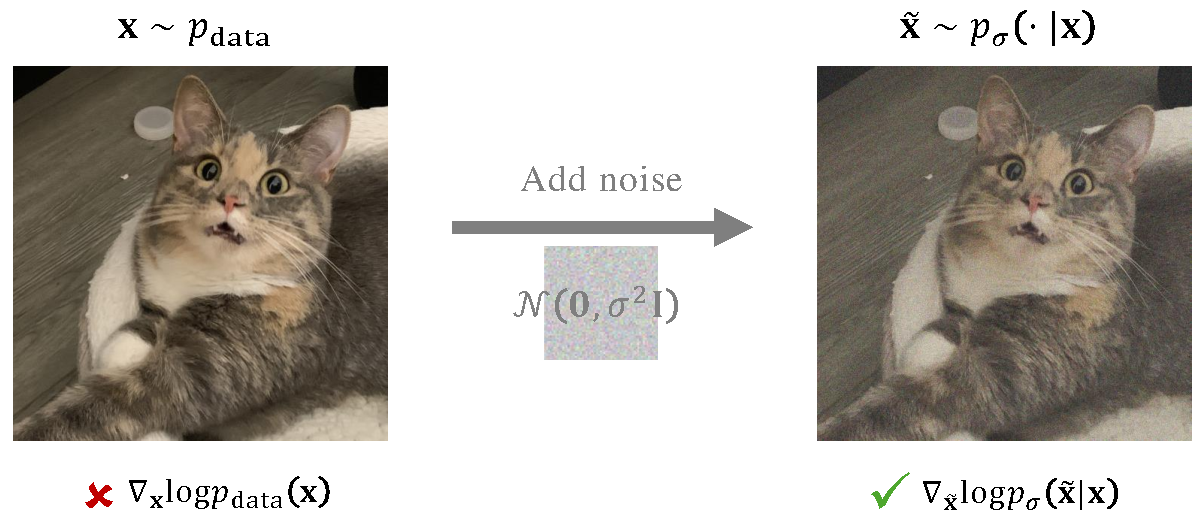
\includegraphics[width=0.8\linewidth]{Images/PartB/dsm-graph.pdf}
    \caption{\textbfs{Illustration of DSM via the conditioning technique.} By perturbing the data distribution $p_{\mathrm{data}}$ with small additive Gaussian noise $\mathcal{N}(\mathbf{0}, \sigma^2 \rmI)$, the resulting conditional distribution $p_{\sigma}(\tilde{\rvx}|\rvx) = \mathcal{N}(\tilde{\rvx}; \rvx, \sigma^2 \rmI)$ admits a closed-form score function.
\figcredit{Created by the authors.}}
    \label{fig:dsm-graph}
\end{figure}


\paragraph{Special Case: Additive Gaussian Noise.} We now consider the common case where Gaussian noise $\mathcal{N}(\mathbf{0}, \sigma^2 \rmI)$ with variance $\sigma^2$ is added to each data point $\rvx \sim p_{\text{data}}$:
\[
\tilde{\rvx} = \rvx + \sigma \bm{\epsilon}, \quad \bm{\epsilon} \sim \mathcal{N}(\mathbf{0}, \rmI),
\]
so that the corrupted data $\tilde{\rvx}$ follows
\[
p_{\sigma}(\tilde{\rvx}|\rvx) = \mathcal{N}(\tilde{\rvx}; \rvx, \sigma^2 \rmI).
\]
In this setting, the conditional score is analytically given by
\[
\nabla_{\tilde{\rvx}} \log p_{\sigma}(\tilde{\rvx}|\rvx) = \frac{\rvx - \tilde{\rvx}}{\sigma^2}.
\]
Hence, the DSM loss simplifies to:
\begin{mdframed}
\begin{align}\label{eq:gaussian-dsm}
\begin{aligned}
    \mathcal{L}_{\text{DSM}}(\bm{\phi}; \sigma) &= \frac{1}{2} \mathbb{E}_{\rvx, \tilde{\rvx}|\rvx} \left[ \norm{\rvs_{\bm{\phi}}(\tilde{\rvx}, \sigma) - \frac{\rvx - \tilde{\rvx}}{\sigma^2}}_2^2 \right] \\
    &= \frac{1}{2} \mathbb{E}_{\rvx, \bm{\epsilon}} \left[ \norm{\rvs_{\bm{\phi}}(\rvx + \sigma \bm{\epsilon}, \sigma) + \frac{\bm{\epsilon}}{\sigma}}_2^2 \right],
\end{aligned}
\end{align}
\end{mdframed}
where $\bm{\epsilon} \sim \mathcal{N}(\mathbf{0}, \rmI)$. This objective forms the core of the (score-based) Diffusion Model. 


At a fixed noise level $\sigma>0$, DSM learns the score of the
Gaussian-smoothed distribution
\[
p_\sigma
=
p_{\mathrm{data}} * \mathcal{N}(\bm{0},\sigma^2\rmI),
\]
rather than the score of $p_{\mathrm{data}}$ itself.
When $\sigma$ is small, the corruption is mild, so $p_\sigma$ still closely
preserves the local structure of the data distribution. Its score therefore
provides a useful direction for moving noisy samples back toward likely data
regions. As $\sigma$ becomes larger, the Gaussian smoothing progressively removes fine
details and merges nearby modes. The corresponding score then captures mainly
coarser, more global structure. This behavior is useful rather than undesirable:
the multi-noise construction in \Cref{sec:SMLD} deliberately combines many noise
levels, using large noise for coarse exploration and small noise for fine
refinement.


To better see why the objective naturally corresponds to a ``denoising'' process,
we expand on the discussion in \Cref{subsec:why-dsm-denoising-tweedie,subsec:why-dsm-denoising-sure}.


% \se{i think it's important to explain why this is denoising. there's also a reasonable intuition where the best way to denoise is to locally maximize the log-likelihood of the nosy distribution. here it's probably good to at least mention Tweedie's formula, and perhaps Stein's unbiased risk estimator.
% probably worth mentioning that the same idea applies to higher order gradients, and in general to any linear operator
% }



\subsection{Sampling} Once we have a trained score model $\rvs_{\bm{\phi}^\times}(\tilde{\rvx}, \sigma)$ at noise level $\sigma$, we generate samples using Langevin dynamics by replacing the true score with the learned model. The update rule is:
\begin{align}\label{eq:score-langevin-emp-dsm}
   \tilde{\rvx}_{n+1} = \tilde{\rvx}_n + \eta \underbrace{\rvs_{\bm{\phi}^\times}(\tilde{\rvx}_n, \sigma)}_{\approx \nabla_{\tilde{\rvx}} \log p_\sigma(\tilde{\rvx}_n)} + \sqrt{2\eta}    \bm{\epsilon}_n, \quad \bm{\epsilon}_n \sim \mathcal{N}(\mathbf{0}, \rmI),
\end{align}
for $n = 0, 1, 2, \dots$, starting from an initial value $\tilde{\rvx}_0$. If $\sigma$ is sufficiently small, then after enough iterations, $\tilde{\rvx}_n$ approximates samples from $p_{\text{data}}$.


\paragraph{Advantages of Noise Injection.}
We additionally remark that, compared to vanilla score matching in \Cref{eq:sm}, injecting Gaussian noise to form $p_\sigma$ (e.g., \Cref{eq:gaussian-dsm}) provides two key advantages~\citep{song2019generative}:
\begin{itemize}
  \item \textbfs{Well-Defined Gradients.} The noise perturbs data away from its lower-dimensional manifold, resulting in a distribution $p_\sigma$ with full support in $\mathbb{R}^D$. Consequently, the score function $\nabla_{\tilde{\rvx}} \log p_\sigma(\tilde{\rvx})$ is well-defined everywhere.
  \item \textbfs{Improved Coverage.} The noise smooths out sparse regions between modes, enhancing training signal quality and facilitating Langevin dynamics to traverse low-density regions more effectively.
\end{itemize}


\subsection{Why DSM is Denoising: Tweedie's Formula}\label{subsec:why-dsm-denoising-tweedie}

We begin with \emph{Tweedie's formula}~\citep{efron2011tweedie}, which provides a principled basis for denoising from noisy observations alone.
Concretely, it states that: given a single Gaussian–corrupted observation $\tilde{\rvx}\sim\mathcal N(\,\cdot\,;\alpha\rvx,\sigma^2\mathrm{I})$  from an unknown $\rvx \sim p_{\mathrm{data}}$, a denoised estimate (the
average over all plausible clean signals given $\tilde{\rvx}$) is obtained by nudging
$\tilde{\rvx}$ a step of size $\sigma^2$ in the direction of the score
$\nabla_{\tilde{\rvx}}\log p_\sigma(\tilde{\rvx})$ of its noisy marginal defined as:
\[
p_\sigma(\tilde{\rvx}):= \int \mathcal{N}(\tilde{\rvx};\alpha \rvx,\sigma^2\mathrm{I})p_{\mathrm{data}}(\rvx)\diff\rvx.
\]
We present the proposition formally below.
\lemp{Tweedie's Formula}{tweedie}{Assume $\rvx\sim p_{\mathrm{data}}$ and, conditionally on $\rvx$,
$\tilde{\rvx}\sim\mathcal N(\,\cdot\,;\alpha\rvx,\sigma^2\mathrm{I})$ with $\alpha\neq0$. Then Tweedie's formula states
 \begin{align}\label{eq:tweedie} 
 \alpha   \mathbb{E}_{\rvx \sim p(\rvx |\tilde\rvx)}\big[\rvx  \big|  \tilde\rvx\big] = \tilde\rvx + \sigma^2 \nabla_{\tilde\rvx} \log p_\sigma(\tilde\rvx), 
 \end{align} where the expectation is taken over the posterior distribution $p(\rvx |\tilde\rvx)$ of $\rvx$ given  $\tilde\rvx$.
}{
The proof proceeds by computing the score of the marginal
\[
p(\tilde\rvx)=\int p(\tilde\rvx|\rvx)p_{\mathrm{data}}(\rvx)\diff\rvx.
\]
Differentiating under the integral and using the Gaussian form of the
conditional density leads directly to an expression that rearranges into
the desired identity linking the score with the posterior mean. See \Cref{app-sec:tweedie} for details.
}
Tweedie’s formula plays a central role in diffusion models, where multiple layers of noise are introduced as in DDPM. 
It enables the estimation of clean samples from noisy observations via the score function, thereby establishing a fundamental link between score prediction and denoiser:
\begin{equation*}
\underbrace{\mathbb{E} \left[\rvx|\tilde\rvx\right]}_{\substack{\text{denoiser}\\\text{estimated from }\tilde\rvx}}
= \frac{1}{\alpha}\left(\tilde\rvx + \sigma^2 \nabla_{\tilde\rvx} \log p_\sigma(\tilde\rvx)\right).
\end{equation*}

Especially,  a single gradient-ascent step on the noisy log-likelihood with the particular step size $\sigma^2$
is the denoised estimate (the conditional average clean signal). This makes
DSM training and denoising tightly related: if $\rvs_\bphi(\tilde{\rvx})\approx
\nabla_{\tilde{\rvx}}\log p_\sigma(\tilde{\rvx})$ trained from DSM, then
\[
\frac{1}{\alpha}\left(\tilde{\rvx}+\sigma^2 \rvs_\bphi(\tilde{\rvx})\right)
\]
is the denoiser.

\paragraph{(Optional) Higher Order Tweedie's Formula.} The classical Tweedie's formula expresses the posterior mean $\E[\rvx_0|\tilde{\rvx}]$ through the gradient $\nabla_{\tilde{\rvx}}\log p(\tilde{\rvx})$.
Higher order extensions~\citep{meng2021estimating} express the posterior covariance and higher cumulants through higher derivatives of $\log p(\tilde{\rvx})$.

\subparagraph{Exponential Family Setup with the Log-Normalizer $\lambda(\tilde{\rvx})$.}
Assume the conditional law of $\tilde{\rvx}$ given a latent natural parameter $\boldsymbol\eta\in\R^D$ belongs to a natural exponential family written as
\[
q_\sigma(\tilde{\rvx}|\boldsymbol\eta)
=\exp\!\big(\boldsymbol\eta^\top \tilde{\rvx}-\psi(\boldsymbol\eta)\big)\,q_0(\tilde{\rvx}).
\]
Here $q_0(\tilde{\rvx})$ is the \emph{base measure}, namely the part that does not depend on $\boldsymbol\eta$; for additive Gaussian noise with variance $\sigma^2\rmI$ it equals $(2\pi\sigma^2)^{-D/2}\exp(-\|\tilde{\rvx}\|^2/2\sigma^2)$.
Let $p(\boldsymbol\eta)$ be the pre-defined distribution of the latent natural parameter, which can be viewed as the reparameterized clean-data distribution (for Gaussian location, $\boldsymbol\eta=\rvx/\sigma^2$).
The observed noisy marginal is
\[
p_\sigma(\tilde{\rvx})=\int q_\sigma(\tilde{\rvx}|\boldsymbol\eta)\,p(\boldsymbol\eta)\diff\boldsymbol\eta.
\]
Define the \emph{log-partition} (log-normalizer) in $\tilde{\rvx}$ by
\[
\lambda(\tilde{\rvx}) := \log p_\sigma(\tilde{\rvx})-\log q_0(\tilde{\rvx}).
\]
Then the posterior of $\boldsymbol\eta$ given $\tilde{\rvx}$ is
\[
p(\boldsymbol\eta|\tilde{\rvx})
\ \propto\
\exp\!\big(\boldsymbol\eta^\top \tilde{\rvx}-\psi(\boldsymbol\eta)-\lambda(\tilde{\rvx})\big)\,p(\boldsymbol\eta),
\]
which shows that, as a function of $\tilde{\rvx}$, the posterior has exponential-family form with natural parameter $\tilde{\rvx}$, sufficient statistic $\boldsymbol\eta$, and log-partition  $\lambda(\tilde{\rvx})$.

\subparagraph{Derivatives of $\lambda$ Produce Posterior Cumulants.}
Two simple rules are at play.
First, normalization: for every $\tilde{\rvx}$,
\[
\int \exp\!\big(\boldsymbol\eta^\top \tilde{\rvx}-\psi(\boldsymbol\eta)-\lambda(\tilde{\rvx})\big)\,p(\boldsymbol\eta)\diff\boldsymbol\eta
=1.
\]
Differentiating this identity with respect to $\tilde{\rvx}$ brings down powers of $\boldsymbol\eta$ from the exponential and derivatives of $\lambda(\tilde{\rvx})$; setting the result to zero yields equalities between derivatives of $\lambda$ and posterior moments of $\boldsymbol\eta$.
Second, a standard property of exponential families: the log-partition is the cumulant generating function of the sufficient statistic.
Therefore
\[
\nabla_{\tilde{\rvx}}\lambda(\tilde{\rvx})=\E[\boldsymbol\eta|\tilde{\rvx}],\quad
\nabla_{\tilde{\rvx}}^{2}\lambda(\tilde{\rvx})=\Cov[\boldsymbol\eta|\tilde{\rvx}],\quad
\nabla_{\tilde{\rvx}}^{(k)}\lambda(\tilde{\rvx})=\kappa_k(\boldsymbol\eta|\tilde{\rvx})\quad(k\ge 3),
\]
where $\kappa_k$ are the \emph{conditional cumulants} of order $k$ of the random vector $\boldsymbol\eta$ given $\tilde{\rvx}$, obtained via the standard moment–cumulant relations.


These are the higher order Tweedie's formulas.
Specializing to the Gaussian location model with $\boldsymbol\eta=\rvx/\sigma^2$ yields the familiar forms in terms of derivatives of $\log p_\sigma(\tilde{\rvx})$:
\[
\E[\rvx|\tilde{\rvx}]
=\tilde{\rvx}+\sigma^2\nabla_{\tilde{\rvx}}\log p_\sigma(\tilde{\rvx}),
\qquad
\Cov[\rvx|\tilde{\rvx}]
=\sigma^2\mathrm I+\sigma^4\nabla_{\tilde{\rvx}}^{2}\log p_\sigma(\tilde{\rvx}),
\]
and higher cumulants scale with higher derivatives of $\log p_\sigma(\tilde{\rvx})$.


Several studies have explored training neural networks to estimate higher order scores~\citep{meng2021estimating,lu2022maximum,lai2023fp}. In contrast, our aim is to clarify their relationship with statistical quantities, and we refer the reader to these works for methodological details.

\subsection{(Optional) Why DSM is Denoising: SURE}\label{subsec:why-dsm-denoising-sure}


\paragraph{SURE (Stein’s Unbiased Risk Estimator).}
At a high level, Stein’s Unbiased Risk Estimator (SURE) is a technique that allows one to 
estimate the mean squared error (MSE) of a denoiser $\rmD$ \emph{without knowing the clean signal}. 
In other words, SURE provides a way to select or train denoisers when only noisy data are available.

For clarity, consider the additive Gaussian noise setting:
\[
\tilde{\rvx} = \rvx + \sigma \bm{\epsilon}, 
\qquad \bm{\epsilon} \sim \mathcal{N}(\mathbf{0},\rmI),
\]
where $\rvx \in \R^D$ is the unknown clean signal and $\tilde{\rvx}$ is the observed noisy version. 
A denoiser is any (weakly differentiable) mapping $\rmD:\R^D \to \R^D$ that produces an estimate $\rmD(\tilde{\rvx})$ of $\rvx$.

The natural quality measure is the conditional MSE
\[
R(\rmD;\rvx) := \E_{\tilde{\rvx}|\rvx}\left[\|\rmD(\tilde{\rvx})-\rvx\|_2^2 \,\big|\, \rvx\right].
\]
This quantity depends on the unknown ground truth $\rvx$, and therefore cannot be computed directly. 
Stein’s identity (see \Cref{app-sec:stein-identity}), however, yields the following \emph{observable} surrogate:
\begin{align}\label{eq:sure-obj}
    \mathrm{SURE}(\rmD;\tilde{\rvx})
= \|\rmD(\tilde{\rvx})-\tilde{\rvx}\|_2^2
+ 2\sigma^2\,\nabla_{\tilde{\rvx}}\cdot \rmD(\tilde{\rvx})
- D\sigma^2,
\end{align}
where $\nabla_{\tilde{\rvx}}\cdot \rmD(\tilde{\rvx})$ denotes the divergence of $\rmD$. 
We emphasize that $\mathrm{SURE}(\rmD;\tilde{\rvx})$ requires only the noisy observation $\tilde\rvx$, not the clean $\rvx$.

Intuitively, $\mathrm{SURE}$ consists of two parts that complement each other. 
The term $\|\rmD(\tilde{\rvx})-\tilde{\rvx}\|^2$ measures how far the denoiser’s output is from the noisy input; 
by itself this underestimates the true error since $\tilde{\rvx}$ is already corrupted. 
The divergence term acts as a correction: it captures how sensitive the denoiser is to small perturbations in its input, 
effectively accounting for the variance introduced by the noise.


Importantly, for any fixed but unknown $\rvx$,
\[
\E_{\tilde{\rvx}|\rvx}\left[\mathrm{SURE}(\rmD;\rvx+\sigma\beps) \,\big|\, \rvx\right]
= R(\rmD;\rvx),
\]
where the expectation is over the Gaussian noise $\beps\sim\mathcal{N}(\bm{0},\rmI)$. Thus, minimizing SURE (in expectation or empirically) is equivalent to minimizing the true MSE, 
while relying only on noisy data. 
In practice, averaging $\mathrm{SURE}$ over both $\rvx\sim p_{\mathrm{data}}$ and the corruption noise $\beps$ 
yields an unbiased estimate of the global MSE risk.

\paragraph{Link to Tweedie’s Formula and Bayes Optimality.}
Let $p_\sigma(\tilde{\rvx}) = \big(p_{\mathrm{data}} * \mathcal{N}(\mathbf{0}, \sigma^2 \rmI)\big)(\tilde{\rvx})$ denote the noisy marginal considered in this section.


SURE is an unbiased estimator of the mean squared error with respect to the noise, conditional on $\rvx$:
\[
\mathbb{E}_{\tilde{\rvx}| \rvx}\!\big[\mathrm{SURE}(\rmD; \tilde{\rvx})\big]
=
\mathbb{E}_{\tilde{\rvx}| \rvx}\!\big[\|\rmD(\tilde{\rvx})-\rvx\|^2\big].
\]
Hence minimizing the expected SURE equals minimizing the Bayes risk
$\mathbb{E}_{(\rvx, \tilde{\rvx})}\big[\|\rmD(\tilde{\rvx})-\rvx\|^2\big]
=\mathbb{E}_{\tilde{\rvx}}\!\big[\mathbb{E}_{\rvx| \tilde{\rvx}}\!\big[\|\rmD(\tilde{\rvx})-\rvx\|^2\big]\big]$ by the law of total expectation (tower property). This decomposition yields a pointwise optimization: for almost every $\tilde{\rvx}$,
\[
\rmD^*(\tilde{\rvx})
=\arg\min_{\mathbf z}\ \mathbb{E}_{\rvx| \tilde{\rvx}}\!\big[\|\mathbf z-\rvx\|^2\big]
=\mathbb{E}[\rvx| \tilde{\rvx}].
\]
Therefore the SURE-optimal denoiser coincides with the Bayes estimator in \Cref{subsec:why-dsm-denoising-tweedie}, and by Tweedie’s identity:
\begin{align}\label{eq:sure-tweedie-denoiser}
    \rmD^*(\tilde{\rvx})=\mathbb{E}[\rvx| \tilde{\rvx}]=\tilde{\rvx}+\sigma^2\nabla_{\tilde{\rvx}}\log p_\sigma(\tilde{\rvx}).
\end{align}




\paragraph{Relationship of SURE and Score Matching.}
The identity in \Cref{eq:sure-tweedie-denoiser} motivates parameterizing the denoiser $\rmD$ via a score field:
\[
\rmD(\tilde{\rvx})=\tilde{\rvx}+\sigma^2\rvs_{\bm\phi}(\tilde{\rvx}, \sigma),
\]
with $\rvs_{\bm\phi}(\cdot, \sigma)$ meant to approximate the noisy score
$\nabla_{\tilde{\rvx}}\log p_\sigma(\cdot)$.
Plugging  $\rmD(\tilde{\rvx})=\tilde{\rvx}+\sigma^2 \rvs_{\bm\phi}(\tilde{\rvx}, \sigma)$ in \Cref{eq:sure-obj} gives
\[
\frac{1}{2\sigma^4}\,\mathrm{SURE}(\rmD;\tilde{\rvx})
=
\Tr\!\big(\nabla_{\tilde{\rvx}} s_{\bm\phi}(\tilde{\rvx}, \sigma)\big)
+\tfrac12\|\rvs_{\bm\phi}(\tilde{\rvx}, \sigma)\|_2^2
+\text{const}(\sigma).
\]
Therefore, taking expectation with respect to $\tilde{\rvx}\sim p_\sigma$, minimizing SURE is
equivalent (up to an additive constant) to minimizing Hyv\"arinen’s alternative
score matching objective at noise level $\sigma$, with the expectation taken under $p_\sigma$ (see \Cref{eq:sm-alternative}).
Consequently, both objectives share the same minimizer, namely the denoiser in \Cref{eq:sure-tweedie-denoiser}.



\subsection{(Optional) Generalized Score Matching}


\paragraph{Motivation.}
Classical score matching, denoising score matching, and higher order variants all target
\[
\frac{\mathcal L p(\rvx)}{p(\rvx)},\quad\text{for some density } p
\]
with a linear operator $\mathcal L$ acting on the density. 
In the classical case $\mathcal L=\nabla_{\rvx}$, this gives 
\[
\nabla_{\rvx}\log p(\rvx) = \frac{\nabla_{\rvx} p(\rvx)}{p(\rvx)}
\]
The $\frac{\mathcal L p}{p}$ structure allows integration by parts to remove normalizing constants, yielding a tractable objective that depends only on samples from $p$ and the learned field $\rvs_\bphi$.
This viewpoint motivates the generalized score matching framework.

\paragraph{Generalized Fisher Divergence.}
Let $p$ be the data distribution and $q$ any model distribution.
For a linear operator $\mathcal L$ on scalar functions of $\rvx$, define the generalized Fisher divergence
\[
\mathcal D_{\mathcal L}(p \,\|\, q)
:= \int p(\rvx) 
\left\|
\frac{\mathcal L p(\rvx)}{p(\rvx)}
-
\frac{\mathcal L q(\rvx)}{q(\rvx)}
\right\|_2^2 \diff \rvx.
\]
If $\mathcal L$ is \emph{complete}, i.e., 
\[
\frac{\mathcal L p_1}{p_1}=\frac{\mathcal L p_2}{p_2} \text{ a.e.}\quad \text{implies}\quad p_1=p_2 \text{ a.e.,}
\]
then $\mathcal D_{\mathcal L}(p \,\|\, q)=0$ identifies $q=p$.
For $\mathcal L=\nabla_{\tilde\rvx}$ this recovers the classical Fisher divergence (see \Cref{eq:fisher}).

\paragraph{Score Parameterization.}
In practice we do not model a normalized density $q$.
Instead, we directly parameterize a vector field $\rvs_\bphi(\rvx)$ to approximate the generalized score $\frac{\mathcal L p(\rvx)}{p(\rvx)}$.
Consider
\[
\mathcal D_{\mathcal L}\!\left(p \,\|\, \rvs_\bphi\right)
:= \mathbb E_{\rvx\sim p}\!\left[\left\|\,\rvs_\bphi(\rvx) - \frac{\mathcal L p(\rvx)}{p(\rvx)}\right\|_2^2\right].
\]
Although $\frac{\mathcal L p(\rvx)}{p(\rvx)}$ is unknown, ``integration by parts'' makes the loss depend only on $\rvs_\bphi$.
Let $\mathcal L^\dagger$ be the adjoint of $\mathcal L$, defined by
\[
\int \big(\mathcal L f\big)^\top g
= \int f\,(\mathcal L^\dagger g)
\quad\text{for all test functions } f,g,
\]
which formally “moves” $\mathcal L$ across the integral when boundary terms vanish.
Expanding the square and applying this identity yields the tractable objective
\[
\mathcal L_{\text{GSM}}(\bphi)
= \mathbb E_{\rvx\sim p}\!\left[
\frac{1}{2}\,\|\rvs_\bphi(\rvx)\|_2^2
-
\big(\mathcal L^\dagger \rvs_\bphi\big)(\rvx)
\right] + \text{const},
\]
where the constant does not depend on $\bphi$. We use $p$ only through expectations, so the generalized score matching loss admits an empirical estimator from training data, exactly as in classical score matching.

For $\mathcal L=\nabla$ we have $\mathcal L^\dagger=-\nabla\!\,\cdot$, which recovers Hyv\"arinen’s score matching objective $\mathbb E_p\!\big[\tfrac{1}{2}\|\rvs_\bphi\|_2^2 + \nabla\!\cdot \rvs_\bphi\big]$ in \Cref{eq:sm-alternative}.

\paragraph{Examples of Operators.}
\begin{itemize}
\item \textbfs{Classical Score Matching.} Consider $\mathcal L = \nabla_{\rvx}$. 
Then the generalized score reduces to the classical score function
\[
\frac{\mathcal L p(\rvx)}{p(\rvx)}
= \nabla_{\rvx}\log p(\rvx).
\]
\item \textbfs{Denoising Score Matching.}
For additive Gaussian noise, define the operator
\[
(\mathcal L f)(\tilde{\rvx})
= \tilde{\rvx}\,f(\tilde{\rvx}) + \sigma^2\nabla_{\tilde{\rvx}} f(\tilde{\rvx}).
\]
Then
\[
\frac{\mathcal L p_\sigma(\tilde{\rvx})}{p_\sigma(\tilde{\rvx})}
= \tilde{\rvx} + \sigma^2\nabla_{\tilde{\rvx}}\log p_\sigma(\tilde{\rvx})
= \mathbb E[\rvx_0|\tilde{\rvx}],
\]
with
\[
p_\sigma(\tilde\rvx)
:=
\int
\mathcal{N}(\tilde\rvx;\rvx_0,\sigma^2\rmI)
\,p_{\mathrm{data}}(\rvx_0)\,\diff\rvx_0,
\qquad
\tilde\rvx=\rvx_0+\sigma\beps.
\]
This is exactly Tweedie's identity for additive Gaussian noise. Minimizing
$\mathcal{L}_{\mathrm{GSM}}$ with this operator therefore trains
$\rvs_{\bphi}$ to approximate the posterior-mean denoiser. If one instead uses
a scaled Gaussian location model
$\tilde\rvx=\alpha\rvx_0+\sigma\beps$, the corresponding identity contains the
factor $\alpha$ as in \Cref{eq:tweedie}.



\item \textbfs{Higher Order Targets.}
Stacking derivatives inside $\mathcal L$ exposes $\nabla^2\log p$ and higher derivatives, which align with posterior covariance and higher order cumulants.
\end{itemize}


\paragraph{Extensions and Use Cases.}
Generalized score matching extends beyond continuous variables to discrete settings, including language modeling \citep{meng2022concrete,lou2024discrete}. It also motivates score inspired training that yields denoising style objectives. This operator view unifies a range of objectives, admits empirical estimation from data, and offers a general principle for designing loss functions through suitable choices of $\mathcal L$.





\clearpage
\newpage


\section{\texorpdfstring{Multi-Noise Levels of Denoising Score Matching (NCSN)}{Multi-Noise Levels of Denoising Score Matching (NCSN)}}\label{sec:SMLD}

\subsection{Motivation}
Adding Gaussian noise with a single fixed variance to the data distribution smooths it to a certain extent, but training a score-based model at only one noise level introduces key limitations. At low levels of injected noise, Langevin dynamics struggles to traverse modes in multi-modal distributions due to vanishing gradients in low-density regions. In contrast, at high noise levels, sampling becomes easier, but the model captures only coarse structures, resulting in blurry samples that lack fine detail. Furthermore, Langevin dynamics can be slow to converge or even fail in high-dimensional spaces. Since it depends on the gradient of the log-density for guidance, poor initialization, particularly in plateau regions or near saddle points, can impede exploration or cause the sampler to get trapped in a single mode.


\begin{figure}[ht!]
    \centering
    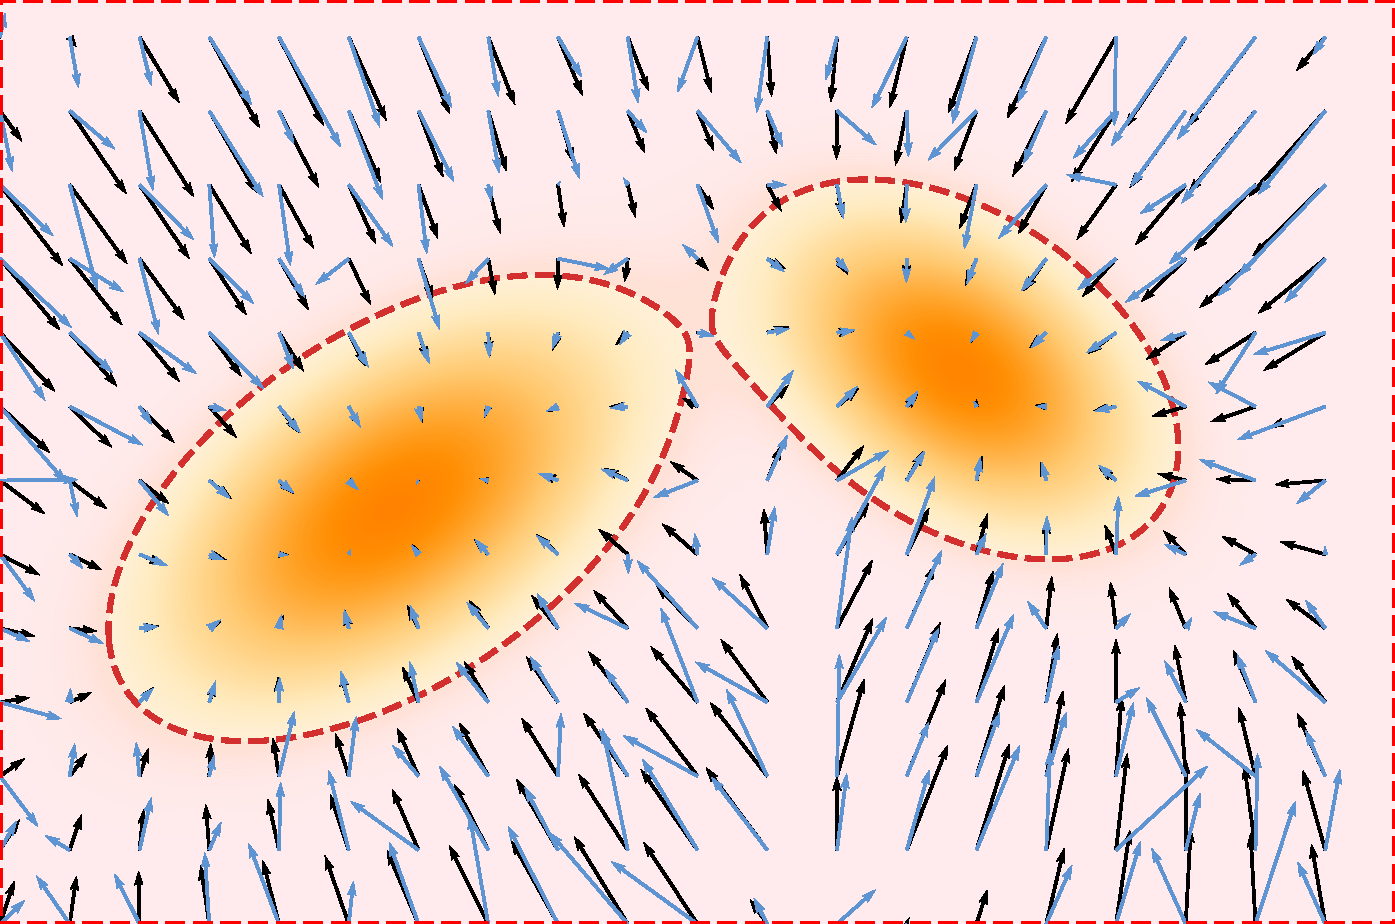
\includegraphics[width=0.85\linewidth]{Images/PartB/score_function_acc.pdf}
    \caption{\textbfs{Illustration of SM inaccuracy (revisiting \Cref{fig:sm-illustration}).} the red region indicates low-density areas with potentially inaccurate score estimates due to limited sample coverage, while high-density regions tend to yield more accurate estimates. \figcredit{Created by the authors.}}
    \label{fig:sm-acc-illustration}
\end{figure}


To address these challenges, \citet{song2019generative} propose injecting Gaussian noise at multiple levels into the data distribution and jointly training a noise-conditional score network (NCSN) to estimate score functions across a range of noise scales. During generation, Langevin dynamics is applied in a noise-annealed fashion: beginning with high-noise levels to enable coarse exploration, and gradually refining toward low-noise levels to recover fine details. 




\begin{figure}[th]
    \centering
    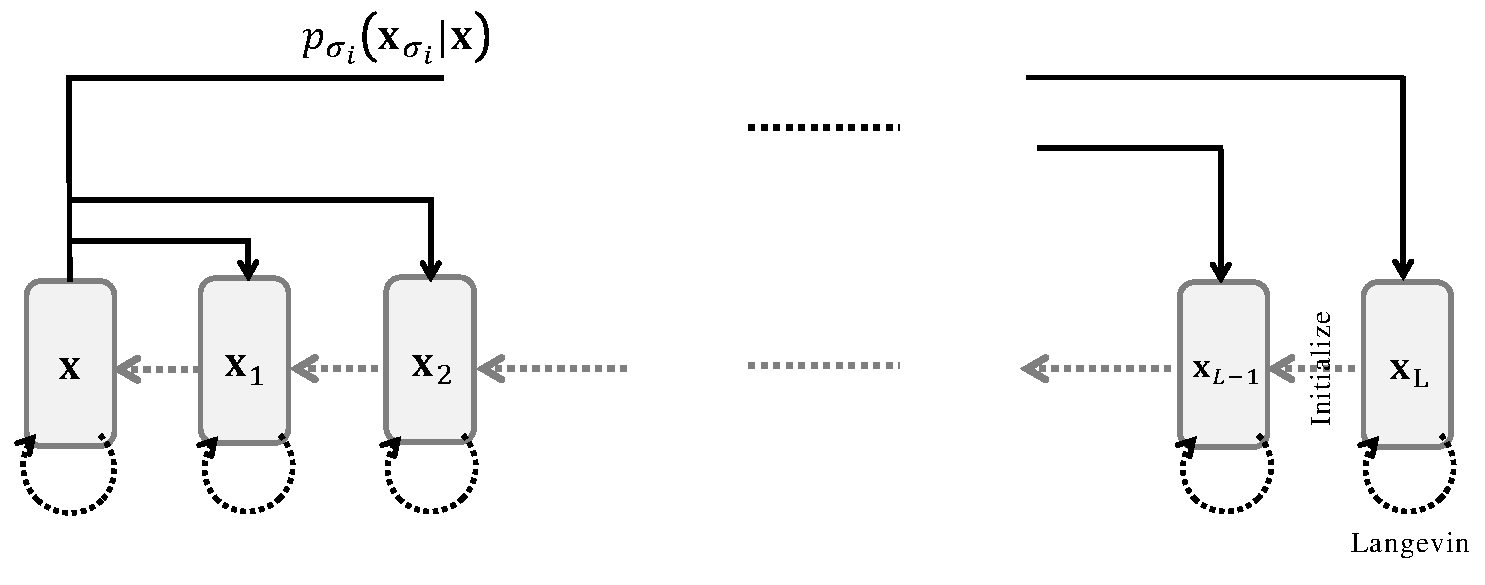
\includegraphics[width=0.95\linewidth]{Images/PartB/ncsn-graph.pdf}
    \caption{\textbfs{Illustration of NCSN.} The forward process perturbs the data with multiple levels of additive Gaussian noise $p_{\sigma}(\rvx_{\sigma} | \rvx)$. Generation proceeds (in dash lines) via Langevin sampling at each noise level, using the result from the current level to initialize sampling at the next lower variance. \figcredit{Created by the authors.}}
    \label{fig:smld-ddpm-graphical-model}
\end{figure}


\subsection{Training}
To overcome the limitations of score-based models trained at a single noise level, \citet{song2019generative} propose adding Gaussian noise at multiple levels to the data distribution. Specifically, a sequence of $L$ noise levels $\{\sigma_i\}_{i=1}^L$ is chosen such that
\[
0 < \sigma_1 < \sigma_2 < \cdots < \sigma_L,
\]
where $\sigma_1$ is small enough to preserve most of the data's fine details, and $\sigma_L$ is large enough to sufficiently smooth the distribution, facilitating easier training.

Each noisy sample is constructed by perturbing a clean data point $\rvx \sim p_{\text{data}}$ as $\rvx_{\sigma} = \rvx + \sigma \bm{\epsilon}$ with $ \bm{\epsilon} \sim \mathcal{N}(\bm{0}, \rmI)$. This defines the  
\vspace{-0.4cm}
\subparagraph{Perturbation Kernel:}
\[
p_{\sigma}(\rvx_{\sigma} | \rvx) := \mathcal{N}(\rvx_{\sigma}; \rvx, \sigma^2 \rmI),
\]
which induces the  
\vspace{-0.4cm}
\subparagraph{Marginal Distribution:}
\[
p_\sigma(\rvx_{\sigma}) = \int p_{\sigma} (\rvx_{\sigma} | \rvx)    p_{\text{data}}(\rvx) \diff \rvx,
\]
at each noise level $\sigma$. It presents the Gaussian smoothed data distribution.

\paragraph{Training Objective of NCSN.}

The goal is to train a noise-conditional score network $\rvs_{\bm{\phi}}(\rvx, \sigma)$ to estimate the score function $\nabla_{\rvx} \log p_\sigma(\rvx)$ for all $\sigma \in \{\sigma_i\}_{i=1}^L$. This is achieved by minimizing the DSM objective across all noise levels:
\begin{align}\label{eq:nscn}
\mathcal{L}_{\text{NCSN}}(\bm{\phi}) := \sum_{i=1}^{L} \lambda(\sigma_i)   \mathcal{L}_{\text{DSM}}(\bm{\phi}; \sigma_i),
\end{align}
where
\begin{align*}
\mathcal{L}_{\text{DSM}}(\bm{\phi}; \sigma) 
= \frac{1}{2} \mathbb{E}_{\rvx \sim p_{\text{data}}(\rvx),   \tilde{\rvx} \sim p_{\sigma}(\tilde{\rvx} | \rvx)} 
\left[ \norm{\rvs_{\bm{\phi}}(\tilde{\rvx}, \sigma) - \left( \frac{\rvx - \tilde{\rvx}}{\sigma^2} \right)}_2^2 \right],
\end{align*}
and $\lambda(\sigma_i)>0$ is a weighting function for each scale.

Minimizing this objective yields the score model $\rvs^*(\rvx, \sigma)$ that recovers the true score at each noise level:
\[
\rvs^*(\cdot, \sigma) = \nabla_{\rvx} \log p_\sigma(\cdot),  \quad \text{for all } \sigma \in \{\sigma_i\}_{i=1}^L,
\]
as it is essentially DSM minimization (see Theorem~\ref{thm:sm-dsm}).
% \se{discuss replationship with ddpm loss}


\paragraph{Relationship with DDPM Loss.}
Let $\rvx_\sigma=\rvx+\sigma\boldsymbol{\epsilon}$ with $\boldsymbol{\epsilon}\sim\mathcal{N}(\mathbf{0},\mathbf{I})$ and let $p_\sigma$ denote the  marginal distribution. By Tweedie’s formula,
\[
\nabla_{\rvx_\sigma}\log p_\sigma(\rvx_\sigma)
= -\frac{1}{\sigma} \E \left[\boldsymbol{\epsilon} \middle|  \rvx_\sigma\right].
\]
Thus the NCSN optimum is the true score $\rvs^*(\rvx_\sigma,\sigma)=\nabla_{\rvx_\sigma}\log p_\sigma(\rvx_\sigma)$, while the Bayes optimal noise predictor under the DDPM loss \Cref{eq:ddpm-simple-loss} is $\boldsymbol{\epsilon}^*(\rvx_\sigma,\sigma)=\E[\boldsymbol{\epsilon}|\rvx_\sigma]$. They are exactly equivalent via
\[
\rvs^*(\rvx_\sigma,\sigma) = - \frac{1}{\sigma} \boldsymbol{\epsilon}^*(\rvx_\sigma,\sigma),
\qquad
\boldsymbol{\epsilon}^*(\rvx_\sigma,\sigma) = - \sigma \rvs^*(\rvx_\sigma,\sigma).
\]
In the DDPM setting, the noisy sample at step $i$ can be written as
\[
\sigma_i:=\sqrt{1-\bar{\alpha}_i^2},
\qquad
\rvx_i
=
\bar{\alpha}_i\rvx_0+\sigma_i\beps,
\qquad
\beps\sim\mathcal{N}(\bm{0},\rmI).
\]
Therefore, the score and the optimal noise prediction contain the same
information:
\[
\rvs^*(\rvx_i,i)
=
-\frac{1}{\sigma_i}
\E\left[\beps|\rvx_i\right].
\]
In other words, predicting the noise in DDPM is equivalent, up to the known
scale factor $1/\sigma_i$, to predicting the score at noise level $i$.

We will systematically compare and summarize this equivalence of parameterizations in \Cref{ch:all-equivalent}.



\subsection{Sampling} 


\begin{algorithm}[th]
\caption{\label{alg:smld} Annealed Langevin Dynamics}
\begin{algorithmic}[1]
\Require Trained score $\rvs_{\bm{\phi}^\times}(\cdot,\sigma_\ell)$,
step sizes $\eta_\ell$, and Langevin iteration budgets $N_\ell$
for each noise level $\ell=L,\ldots,1$; initialization distribution
$p_{\mathrm{init}}$
\State $\rvx \sim p_{\mathrm{init}}$
\Statex\Comment{Initialize from unstructured noise at the largest noise level}
\For{$\ell=L,L-1,\ldots,1$}
    \State $\tilde{\rvx}_0 \gets \rvx$
    \Statex\Comment{Initialize this noise level from the previous level's output}
    \For{$n=0$ \textbf{to} $N_\ell-1$}
        \State $\bm{\epsilon}_n \sim \mathcal{N}(\bm{0},\rmI)$
        \State $\tilde{\rvx}_{n+1}
        \gets
        \tilde{\rvx}_n
        +\eta_\ell
        \rvs_{\bm{\phi}^\times}(\tilde{\rvx}_n,\sigma_\ell)
        +\sqrt{2\eta_\ell}\,\bm{\epsilon}_n$
    \EndFor
    \State $\rvx \gets \tilde{\rvx}_{N_\ell}$
    \Statex\Comment{Pass the final state to the next smaller noise level, if any}
\EndFor
\Ensure $\rvx$
\end{algorithmic}
\end{algorithm}


With trained score networks available at multiple noise levels
\[
\rvs_{\bm{\phi}^\times}(\cdot, \sigma_1), \quad\rvs_{\bm{\phi}^\times}(\cdot, \sigma_2), \quad \cdots, \quad \rvs_{\bm{\phi}^\times}(\cdot, \sigma_{L-1}), \quad    \rvs_{\bm{\phi}^\times}(\cdot, \sigma_L),
\]
% \se{this notation is weird}\jcc{do you meant the notation of $\bm{\phi}^\times$ is weird, which i was thoroughly using $\bm{\phi}^\times$ to denote a trained network? }
the sampling procedure known as \emph{annealed Langevin dynamics}~\citep{song2019generative} generates data by progressively denoising from a high noise level $\sigma_L$ down to a low noise level $\sigma_1 \approx 0$.

With trained scores at noise levels
$0<\sigma_1<\cdots<\sigma_L$, annealed Langevin dynamics generates samples by
moving gradually from high noise to low noise.
Starting from a simple initialization
$\rvx\sim p_{\mathrm{init}}$, it first applies Langevin dynamics at the largest
noise level $\sigma_L$, whose score
$\rvs_{\bm{\phi}^\times}(\cdot,\sigma_L)$ guides the samples toward the
corresponding smoothed distribution $p_{\sigma_L}$.
The resulting samples are then used to initialize Langevin dynamics at the next
smaller noise level. Repeating this procedure progressively refines the samples
until the smallest noise level $\sigma_1$ is reached.

At each noise level $\sigma_\ell$, Langevin dynamics performs the update
\[
\tilde{\rvx}_{n+1}
=
\tilde{\rvx}_n
+
\eta_\ell
\rvs_{\bm{\phi}^\times}(\tilde{\rvx}_n,\sigma_\ell)
+
\sqrt{2\eta_\ell}\,\bm{\epsilon}_n,
\qquad
\bm{\epsilon}_n\sim\mathcal{N}(\bm{0},\rmI),
\]
where the output from the previous noise level provides the initialization
$\tilde{\rvx}_0$.
A common choice is to scale the step size with the noise level as
\[
\eta_\ell
=
\delta\frac{\sigma_\ell^2}{\sigma_1^2},
\qquad
\delta>0.
\]
The algorithm performs Langevin updates at every noise level, including
$\sigma_1$, so the final sample is obtained after refinement at the smallest
noise level. \Cref{alg:smld} summarizes the procedure.

The initial distribution $p_{\mathrm{init}}$ simply provides a starting point
for the Markov chain. At the largest noise level, Langevin dynamics moves this
initial distribution toward $p_{\sigma_L}$, after which the successive noise
levels gradually guide the samples toward increasingly less smoothed versions
of the data distribution.

\paragraph{Slow Sampling Speed of NCSN.}
NCSN generates samples using annealed MCMC (commonly Langevin dynamics) across noise scales $\{\sigma_i\}_{i=1}^L$.  
For each scale $\sigma_i$, it performs $K$ iterative updates of the form ``update $\tilde{\mathbf{x}}_n$ using the score $\rvs_{\bm{\phi}^\times}(\tilde{\mathbf{x}}_n,\sigma_i)$ plus a small random perturbation'', each requiring a forward pass through the score network. Two factors necessitate large $L \times K$:  
\begin{enumerate}
    \item[(i)] \textbfs{Local Accuracy and Stability:} the learned score is reliable only for small perturbations, requiring small step sizes and many iterations per noise level to avoid bias or instability;
    \item[(ii)] \textbfs{Slow Mixing in High Dimensions:} local MCMC moves explore multimodal, high-dimensional targets inefficiently, demanding many iterations to reach typical data regions.
\end{enumerate}
Because updates are strictly sequential (each iteration depends on the previous one) and each requires an expensive network evaluation, the overall cost is $\mathcal{O}(L  K)$ sequential network passes, making sampling computationally slow.

% \newpage

% \paragraph{Link Between Fisher Divergence and KL Divergence.} Maximum likelihood fits $q_\bphi$ by minimizing $\mathcal{D}_\mathrm{KL}(p\|q_\bphi)=\mathbb{E}_{p}[\log p-\log q_\bphi]$. Score matching fits $q_\bphi$ by minimizing the Fisher divergence $\mathcal{D}_{\mathrm F}(p\|q_\bphi)=\mathbb{E}_{p} \big[\|\nabla \log p-\nabla \log q_\bphi\|^2\big]$. They agree at the optimum ($p=q_\bphi$) but use different discrepancy measures. The key bridge is that when you smooth both distributions with Gaussian noise, $p_t=p*\mathcal N(\bm{0},t\rmI)$ and $q_t=q_\bphi*\mathcal N(\bm{0},t\rmI)$, the KL decreases along the noise scale at a rate given by Fisher:
% \[
% \frac{\diff}{\diff t}\mathcal{D}_\mathrm{KL}(p_t\|q_t)=-\tfrac12 \mathcal{D}_{\mathrm F}(p_t\|q_t).
% \]
% So Fisher is the instantaneous decay rate of KL under Gaussian smoothing. Moreover, for many smooth, near Gaussian targets (those satisfying a log Sobolev inequality), minimizing $\mathcal{D}_{\mathrm F}(p\|q_\bphi)$ controls $\mathcal{D}_\mathrm{KL}(p\|q_\bphi)$ via a bound like $\mathcal{D}_\mathrm{KL}(p\|q_\bphi)\lesssim \mathcal{D}_{\mathrm F}(p\|q_\bphi)$. In practice, this explains why score matching (and its denoising version used in diffusion models) can learn models with good likelihood while avoiding the intractable partition function: it matches scores directly, which do not depend on normalization, yet it still pushes down KL through the smoothing identity.



\clearpage
\newpage

\section{Summary: A Comparative View of NCSN and DDPM}

We begin by comparing the graphical models of NCSN and DDPM in \Cref{fig:smld-ddpm-graphical-model}, with key differences and similarities summarized in \Cref{tb:comparison-smld-ddpm}.


\begin{table}[th]
  \caption{Comparisons of NCSN and DDPM}
  \small
  \centering
  \resizebox{\textwidth}{!}{
  \begin{tabular}{cccc}
     \toprule
    
         &   \textbfs{NCSN}   & \textbfs{DDPM}  \\
        \midrule
    $\rvx_{i+1}|\rvx_{i}$ & Derive as $\rvx_{i+1} =  \rvx_i + \sqrt{\sigma^2_{i+1}-\sigma^2_{i}}\bm{\epsilon}$   &  \cc{15}Define as $\rvx_{i+1} = \sqrt{1-\beta_{i}} \rvx_{i} + \sqrt{\beta_{i}}\bm{\epsilon}$  \\
      $\rvx_{i}|\rvx$   & \cc{15}Define as $\rvx_{i} =  \rvx + \sigma_{i}\bm{\epsilon}$
       &  Derive as $\rvx_i = \bar{\alpha}_i\rvx + \sqrt{1 - \bar{\alpha}_i^2}\bm{\epsilon}$ \\
   $p_{\text{prior}}$   & $ \mathcal{N}(\bm{0}, \sigma_L^2\rmI)$    &  $\mathcal{N}(\bm{0}, \rmI)$  \\
   \midrule
        Loss 
          &  
        $\mathbb{E}_{i} \mathbb{E}_{p_{\text{data}}(\rvx)} 
        \mathbb{E}_{\bm{\epsilon} \sim \mathcal{N}\left(\mathbf{0}, \rmI\right)}   
    \left[ \norm{\rvs_{\bm{\phi}}(\rvx_i, \sigma_i) +   \frac{\bm{\epsilon}}{\sigma_i}}_2^2 \right] $ 
            &  $      \mathbb{E}_{i}\mathbb{E}_{p_{\text{data}}(\rvx)} \mathbb{E}_{\bm{\epsilon}\sim \mathcal{N}(\bm{0},\rmI)}\left[ \norm{\bm{\epsilon}_{\bm{\phi}}(\rvx_i, i) - \bm{\epsilon}}_2^2 \right]$ \\
    \midrule
     Sampling   & \begin{tabular}{@{}c@{}} Apply Langevin per layer;\\ use output to initialize the next \end{tabular}  &  \begin{tabular}{@{}c@{}}Traversing the Markovian chain with \\ $p_{\bm{\phi}^\times}(\rvx_{i-1} | \rvx_i)$   \end{tabular} \\
 \bottomrule
  \end{tabular}
  }
  \label{tb:comparison-smld-ddpm}
\end{table}

\paragraph{A Shared Bottleneck.}
Despite their different formulations, both NCSN and DDPM rely on dense time discretization. This leads to a critical limitation: sampling often requires hundreds or even thousands of iterations, making generation slow and computationally intensive.

\begin{question}\label{ques:dm-sampling-slow}
    How can we accelerate sampling in diffusion models?
\end{question}

We return to this challenge in \Cref{ch:solvers}, which develops more efficient samplers; \Cref{ch:distillation}, which compresses pretrained diffusion models requiring hundreds of sampling steps into fewer-step student generators; and \Cref{ch:fast-scratch}, which studies how to learn fast few-step generators directly from scratch under diffusion-inspired principles.

% \paragraph{What Lies Ahead?}

% Despite their seemingly different origins, NCSN and DDPM share a strikingly similar high-level philosophy. Both inject noise at multiple levels and train models to progressively denoise, enabling tractable learning through conditioning and effective generation via noise-annealed refinement. This principle of layering stochasticity and learning to reverse it step-by-step provides a powerful foundation for modeling complex data distributions. 

% In the next chapter, \Cref{ch:score-sde}, we step into the continuous-time world, where the boundary between DDPM and NCSN begins to blur, revealing a profound unification at the heart of diffusion modeling.

\newpage

\section{Closing Remarks}\label{sec:ch3_cr}



This chapter has charted a second major path to diffusion models, beginning from the score-based perspective rooted in Energy-Based Models (EBMs). We started by identifying the core challenge of EBMs—the intractable partition function—and introduced the score function, $\nabla_{\mathbf{x}}\log{p(\mathbf{x})}$, as a powerful tool that circumvents this issue entirely.

Our journey led us from classic score matching to its more scalable and robust variant, Denoising Score Matching (DSM). Through DSM, we saw how perturbing data with noise enables a tractable training objective, once again leveraging a conditioning strategy to create a simple regression target. Furthermore, we established a profound connection between score estimation and the act of denoising via Tweedie's formula, which showed that the score provides the precise direction needed to estimate a clean signal from its noisy observation.


This principle was then extended from a single noise level to a \emph{ladder}
of noise levels with Noise Conditional Score Networks (NCSN), which learn a
single score model conditioned on multiple noise scales and generate samples
via annealed Langevin dynamics. The next chapter takes the additional step from
this discrete ladder to a continuum of noise levels through the Score SDE
framework.




This convergence is no coincidence; it hints at a deeper, unified mathematical structure. The limitations of these discrete-time models motivate the need for a more general framework. In the next chapter, we will take this crucial step:
\begin{enumerate}
    \item We will move into a continuous-time perspective, showing that both DDPMs and NCSNs can be elegantly unified as different discretizations of a single, powerful process described by a Stochastic Differential Equation (SDE).
    \item This Score SDE framework will formally connect the variational and score-based views, recasting the problem of generation as one of solving a differential equation.
\end{enumerate}

This unifying lens will not only provide profound theoretical clarity but also unlock a new class of advanced numerical methods designed to tackle the fundamental challenge of slow sampling. 